\newcommand{\NOTESTITLE}{Title of Notes}
\newcommand{\AUTHOR}{Flip Tanedo}
\newcommand{\EMAIL}{{flip.tanedo@ucr.edu}}
\newcommand{\ADDRESS}{ 	Department of Physics \& Astronomy, 
	    				University of  California, Riverside, 
	    				{CA} 92521
	    			  }


%% LaTeX Paper Template, Flip Tanedo (flip.tanedo@ucr.edu)
%% last updated: Dec 2016

\documentclass[12pt]{article}

%%%%%%%%%%%%%%%%%%%%%%%%%%
%%%  COMMON PACKAGES  %%%%
%%%%%%%%%%%%%%%%%%%%%%%%%%

\usepackage{amsmath}
\usepackage{amssymb}
\usepackage{amsfonts}
\usepackage{graphicx}
\usepackage[utf8]{inputenc}	% for inspirehep.net bibs
% Package inputenc Warning: inputenc package ignored with utf8 based engines. 

%%%%%%%%%%%%%%%%%%%%%%%%%%%%%%%%%
%%%  UNUSUAL PACKAGES        %%%%
%%%  Uncomment as necessary. %%%%
%%%%%%%%%%%%%%%%%%%%%%%%%%%%%%%%%

%% MATH AND PHYSICS SYMBOLS
%% ------------------------
\usepackage{slashed}       % \slashed{k}
\usepackage{mathrsfs}      % Weinberg-esque letters
%\usepackage{youngtab}	    % Young Tableaux
\usepackage{pifont}        % check marks
\usepackage{bbm}           % \mathbbm{1} incomp. w/ XeLaTeX 
%\usepackage[normalem]{ulem} % for \sout
\usepackage{cancel}

%% CONTENT FORMAT AND DESIGN
%% -------------------------
\usepackage[dvipsnames]{xcolor}
\usepackage{fancyhdr}		% to put preprint number
\usepackage{lipsum}         % block of text (formatting test)
\usepackage{framed}        % boxed remarks
%\usepackage{subcaption}    % subfigures; subfig depreciated
%\usepackage{paralist}      % compactitem
%\usepackage{appendix}      % subappendices
%\usepackage{cite}          % group cites (conflict: collref)
%\usepackage{tocloft}       % Table of Contents	
%\usepackage{xspace}			% spacing after macros
%\usepackage{listings}      % \begin{lstlisting}, for code
%	\lstset{
%		basicstyle=\ttfamily\footnotesize,
%		breaklines=true,
%		backgroundcolor=\color{gray!15!white}}


%% TABLES IN LaTeX
%% ---------------
\usepackage{booktabs}      % professional tables
\usepackage{nicefrac}      % fractions in tables,
%\usepackage{multirow}      % multirow elements in a table
%\usepackage{arydshln} 	    % dashed lines in arrays

%% Other Packages and Notes
%% ------------------------
\usepackage[font=small]{caption} % caption font is small
\usepackage{float}         % for strict placement e.g. [H]


%% CUSTOM PACKAGES
%% ---------------
% \usepackage{tikzfeynman}   % Flip's rules Feynman Diagrams



%%%%%%%%%%%%%%%%%%%%%%%%%%%%%%
%%%  DOCUMENT PROPERTIES  %%%%
%%%%%%%%%%%%%%%%%%%%%%%%%%%%%%

\usepackage[margin=2cm]{geometry}   % margins
\graphicspath{{figures/}}			% figure folder
\numberwithin{equation}{section}    % set equation numbering

%% References in two columns, smaller
%% http://tex.stackexchange.com/questions/20758/bibliography-in-two-columns-section-title-in-one
\usepackage{multicol}
\usepackage{etoolbox}
\usepackage{relsize}
\patchcmd{\thebibliography}
  {\list}
  {\begin{multicols}{2}\smaller\list}
  {}
  {}
\appto{\endthebibliography}{\end{multicols}}
%
%% Alternative (one column, modify spacing)
%% https://wiki.math.cmu.edu/iki/wiki/tips/20140712-bibtex-spacing.html


% Change list spacing (instead of package paralist)
% from: http://en.wikibooks.org/wiki/LaTeX/List_Structures#Line_spacing
\let\oldenumerate\enumerate
\renewcommand{\enumerate}{
  \oldenumerate
  \setlength{\itemsep}{1pt}
  \setlength{\parskip}{0pt}
  \setlength{\parsep}{0pt}
}

\let\olditemize\itemize
\renewcommand{\itemize}{
  \olditemize
  \setlength{\itemsep}{1pt}
  \setlength{\parskip}{0pt}
  \setlength{\parsep}{0pt}
}


%%%%%%%%%%%%%%%%%%%%%%%%%%%
%%%  (RE)NEW COMMANDS  %%%%
%%%%%%%%%%%%%%%%%%%%%%%%%%%

%% FOR `NOT SHOUTING' CAPS (e.g. acronyms)
%% ---------------------------------------
\newcommand{\acro}[1]{\textsc{\MakeLowercase{#1}}}    

%% COMMON PHYSICS MACROS
%% ---------------------
\renewcommand{\tilde}{\widetilde}   % tilde over characters
\renewcommand{\vec}[1]{\mathbf{#1}} % vectors are boldface
\newcommand{\dbar}{d\mkern-6mu\mathchar'26}    % for d/2pi
\newcommand{\ket}[1]{\left|#1\right\rangle}    % <#1|
\newcommand{\bra}[1]{\left\langle#1\right|}    % |#1>
\newcommand{\Xmark}{\text{\sffamily X}}        % cross out

%% COMMANDS FOR TEMPORARY COMMENTS
%% -------------------------------
\newcommand{\comment}[2]{\textcolor{red}{[\textbf{#1} #2]}}
\newcommand{\flip}[1]{{
	\color{green!50!black} \footnotesize [\textbf{\textsf{Flip}}: \textsf{#1}]
	}}

%% COMMANDS FOR TOP-MATTER
%% -----------------------
\newcommand{\email}[1]{\href{mailto:#1}{#1}}
\newenvironment{institutions}[1][2em]{\begin{list}{}{\setlength\leftmargin{#1}\setlength\rightmargin{#1}}\item[]}{\end{list}}

%% COMMANDS FOR LATEXDIFF
%% ----------------------
%% see http://bit.ly/1M74uwc
\providecommand{\DIFadd}[1]{{\protect\color{blue}#1}} %DIF PREAMBLE
\providecommand{\DIFdel}[1]{{\protect\color{red}\protect\scriptsize{#1}}}

%% REMARK: use latexdiff option --allow-spaces
%% for \frac, ref: http://bit.ly/1iFlujR



%%%%%%%%%%%%%%%%%%%
%%%  HYPERREF  %%%%
%%%%%%%%%%%%%%%%%%%

%% This package has to be at the end; can lead to conflicts

\usepackage[
	colorlinks=true,
	citecolor=green!50!black,
	linkcolor=NavyBlue!75!black,
	urlcolor=green!50!black,
	hypertexnames=false]{hyperref}


%%%%%%%%%%%%%%%%%%%%%
%%%  TITLE DATA  %%%%
%%%%%%%%%%%%%%%%%%%%%

%% PREPRINT NUMBER USING fancyhdr
%% Don't forget to set \thispagestyle{firststyle}
%% ----------------------------------------------
\renewcommand{\headrulewidth}{0pt} 	% no separator
\setlength{\headheight}{15pt} 		% min to avoid fancyhdr warning
\fancypagestyle{firststyle}{
	\rhead{\footnotesize%
%	\texttt{UCR-TR-2017-FLIP-00X}%
	}}

%% TOC overwrites fancyhdr, here's a fix
%% http://tex.stackexchange.com/questions/167828/difficult-with-fancyhdr-and-table-of-contents
\usepackage{etoc}
\renewcommand{\etocaftertitlehook}{\pagestyle{plain}}
\renewcommand{\etocaftertochook}{\thispagestyle{firststyle}}


\begin{document}

%\thispagestyle{empty}		% default if no preprint #
\thispagestyle{firststyle} 	% to include preprint

\begin{center}

    {\huge \bf P231: Methods of Theoretical Physics}

    \vskip .7cm

%% SINGLE AUTHOR FORMAT
%% --------------------
	\textbf{Flip Tanedo} \\
	\texttt{\footnotesize \email{\EMAIL}}
	
  \begin{institutions}[2.25cm]
    \footnotesize
    {\it \ADDRESS }    
    \end{institutions}


\end{center}
















%%%%%%%%%%%%%%%%%%%%%
%%%  ABSTRACT    %%%%
%%%%%%%%%%%%%%%%%%%%%

\begin{abstract}
\noindent 
Notes for P231 based on the 2019 course.
\end{abstract}

%\small
%\setcounter{tocdepth}{2}
%\tableofcontents
%\normalsize


%%%%%%%%%%%%%%%%%%%%%
%%%  THE MEAT    %%%%
%%%%%%%%%%%%%%%%%%%%%

\section{What this course is about}

Physics 231: Methods of Theoretical Physics is a course for first-year physics and astronomy graduate students. It is a `crash course’ in mathematical methods necessary for graduate courses in electrodynamics, quantum mechanics, and statistical mechanics. The style of the course is a boot camp rather than a rigorous theorem--proof mathematics lecture. Where possible, the emphasis is on physical intuition rather than mathematical precision. 

\subsection{Green’s functions}

The primary goal of this course is to use Green’s functions to solve  linear differential equations. The general form of such a differential equation is
\begin{align}
  \mathcal O f(x) = s(x) \ ,
\end{align}
where $\mathcal O$ is some differential operator that encodes some kind of physical dynamics, $s(x)$ is the source of those dynamics, and $f(x)$ is a response that we would like to determine. Colloquially, the Green’s function is the operator $\mathcal O^{-1}$. But what the heck does that even mean? 

We will approach this problem by analogy to linear algebra, where a linear transformation $A$ acting on a vector space can give equations like:
\begin{align}
  A \vec{v} = \vec{w} \ ,
\end{align}
whose solution is
\begin{align}
  \vec{v} = A^{-1} \vec{w} \ .
\end{align}
We will connect the notion of a linear differential operator to a matrix in infinite dimensional space to give a working definition of $\mathcal O^{-1}$. We will then pull out a bag of tricks from complex analysis to formally solve $\mathcal O^{-1}s(x)$ given $\mathcal O$ and $s(x)$. 




\subsection{Mathematical Niceness}

In my personal approach to mathematics in physics, I have found it useful to have the notion of a \textbf{nice} mathematical situation. This is not a formal idea, and it is one of the many things mathematicians find ridiculous about me. But as a physicist, the concept of mathematical \emph{niceness} is helpful. 

The idea is simply that the physical systems that we tend to care about are all \emph{nice}. What that means is that they rarely populate the degenerate `special exceptions’ that mathematicians worry about. Those exceptions may be the difference between a mathematical theorem being true or false for general cases. We rarely care about general cases---we care about the cases that nature seems to populate.

As such, we rarely have to worry about whether a function is smooth, or even the precise details of a perturbation expansion’s radius of convergence. We rarely deal with operators that are not Hermitian. We rarely worry about the existence of orthonormal bases---the spaces in physics are all \emph{nice}. We rarely have to worry about these degenerate cases, and so most of our energy goes toward understanding the mathematical properties of the \emph{nice} cases that describe nature.

Every once in a while, we \emph{do} have to worry about the exceptional cases. Those scenarios are the most interesting of all. That’s when the mathematical formalism that we use to describe physics grabs us by the collar and says, \emph{listen to me---something important is happening and it probably has to do with nature!} Usually this is what happens when a calculation tells us that a physical result is infinite. 

That being said, in this course, we will focus on \emph{nice} functions and \emph{nice} operators and \emph{nice} boundary conditions, etc. For the most part, this is what we need to make progress on our physical models and it’s worth spending our time learning to work with \emph{nice} limits. Leave the degenerate cases to the mathematicians for now. Eventually, though, you may find yourself in a situation where physics demands \emph{not nice} mathematics. In that case---and only when the physics demands it---you will be ready to poke and prod at the mathematical curiosity until the underlying \emph{physics} reason for the not-niceness is apparent.

All this is to say: if you object to this course because we do not start with proofs about open sets or convergence, then you’re missing the point.

\subsection{Physics vs. Mathematics, I}

Let’s make one point clear:
\begin{align}
  \text{Physics} \neq \text{Mathematics} \ .
\end{align}
There are many ways that this is true. Physics is intimately tied to experimental results and empirical science. Physicists will Taylor expand to their hearts’ content---sometimes even when the expansion is not formally justified. Physicists use explicit coordinates, mathematicians abhor this. 

Physicists seek to uncover a truth about \emph{this} universe. We use mathematical formalism to describe the universe. Sometimes the formalism that we need even spurs on developments in formal mathematics. However, let us be clear that our descriptions of the universe are \emph{mathematical models}. Our models have limits of validity: where they are tested, where they break down. 

Sometimes our models will break down in a way that is manifest: the classical potential of an electron orbiting a proton appears to have a divergence when the electron is arbitrarily close to the proton. In fact, quantum mechanically the problem gets worse: if the electron can literally overlap with the proton in some `wavefunctiony’ sense, then there’s some piece of the electron that is hitting the singularity. The solution is that there is additional physics that our description failed to account for.\footnote{If one has not thought about this problem, please do so. What is the new physics that resolves the Coulomb singularity?} 

\subsection{Physics vs. Mathematics, II}

In this class we will write lots of equations. We will use binary relations like $=$ or $\neq$. Sometimes to make a point we’ll write $\cong$ or $\equiv$ or $\dot =$ to mean something like `definition’ or `tautologically equivalent to’ or some other variant of `even more equal than equal.’ 

As physicists, though, the most important binary relation is none of those things. Usually what we really care about is in $\sim$.\footnote{I use this the same way as $\propto$, which is completely different from `approximately.’ $\approx$.} This tells how how something \emph{scales}. If I double a quantity on the right-hand side, how does the quantity on the left-hand side scale? Does it depend linearly? Quadratically? Non-linearly? The answer encodes something important about the underlying physics of the system and lies at the heart of the \emph{imagine a cow is a sphere} joke. 


By the way, implicit in this is the idea that in this class, we will not care about stray factors of 2. As my adviser used to say, if you’re worried about a factor of 2, then your additional homework is to figure out that factor of 2. 

\subsection{Physics vs. Mathematics, III}

There is another way in which physics is different from mathematics, and it is far more prosaic. Quantities in physics have units. We don’t just deal with numbers, we deal with kilograms, electron volts, meters. It turns out that dimensional analysis is a big part of what we do as physicists. 


\section{Dimensional Analysis}

You’ll be surprised how far you can go in physics by thinking deeply about dimensional analysis. Here we’ll only get you started. To go one step further, you may read more about the Buckingham Pi theorem\footnote{\url{https://aapt.scitation.org/doi/10.1119/1.1987069}} or dive into neat applications\footnote{\url{https://aapt.scitation.org/doi/full/10.1119/1.3535586?ver=pdfcov}}\footnote{\url{http://inspirehep.net/record/153032?ln=en}}.

\subsection{Converting Units}

Imagine that you have three apples. This is a number (three) an a unit (apple). The meaning of the unit depends on what you’re using it to measure. For example, if apples are \$1 each, then you could use an apple as a unit of currency. The way to do this is to simply \emph{multiply by one}:
\begin{align}
  (3\text{ apples}) \times \left(\frac{\text{\$ 1}}{\text{apple}}\right)
  &= \$ 3 \ .
\end{align}
We have used the fact that the exchange rate is simply the statement that
\begin{align}
  1\text{ apple} &= \$1
  & \Rightarrow &&
  1 &= \frac{\$ 1}{1\text{ apple}} \ .
\end{align}
You can do a similar thing for [kilo-]calories or any other conversion rate. 


All that matters is that the conversion is constant. Indeed, the constants of nature make very good `exchange rates.' For example, in high-energy physics we like to use \textbf{natural units}. This is the curious statement that
\begin{align}
  \hbar = c = 1 \ .
\end{align}
At face value, this doesn’t make sense. $\hbar$ has units of action, $c$ is a speed, and 1 is dimensionless. However, because nature gives us a \emph{fundamental} unit of action and a \emph{fundamental} unit of speed, we may use them as conversion factors (exchange rates),
\begin{align}
  c = 3 \times 10^{10}~\text{cm}/\text{s} \ .
\end{align}
If $c=1$, then this means
\begin{align}
  1 \text{ s} &=  3 \times 10^{10}~\text{cm} \ .
\end{align}
This, in turn, connects a unit of time to a unit of distance. By measuring time, the constant $c$ automatically gives us an associated distance. The physical relevance of the distance is tied to the nature of the fundamental constant: one second (or `light-second‘) is the distance that a photon travels in one second. Observe that this only works because $c$ is a constant. 

\subsection{Quantifying the units}

We use the notation that a physical quantity $Q$ has \textbf{dimension} $[Q]$ that can be expressed in terms of units of length, mass, and time:
\begin{align}
  [Q] = L^a M^b T^c \ .
\end{align}
The {dimension} is the statement of the powers $a$, $b$, and $c$. You may want to also include units of, say, electric charge. Sticklers may pontificate about whether electric charge formally carries a new unit or not. 

As a simple example, we may want to figure out the units of force. We remember that $\vec{F} = m\vec{a}$, so 
\begin{align}
  [\vec F] &= [m][\vec{a}] = M\times L T^{-2} = L^1 M^1 T^{-2} \ .
\end{align}
Life is even easier in natural units, where $c=1$ means that units of length and time are `the same’ and $\hbar = 1$ means that units of time and energy (mass) are inversely related. In natural units, one typically write $[Q]$ to mean the mass-dimension of a quantity. To revert back to conventional units, one simply multiplies by appropriate factors of $1=c$ and $1=\hbar$. 

\subsection{Usage: Sanity Check}

The simplest use of dimensional analysis is to check your work. It simply does not make sense to ever write
\begin{align}
  1 + (3~\text{cm}) \ .
\end{align}
This does not make sense. You cannot sum together terms of different dimension. Similarly, $\sin(3\text{ cm})$ does not make sense. What about $e^{5~\text{cm}}$? This doesn't make sense because
\begin{align}
  e^x = 1 + x + \frac{1}{2!} x^2 +  \cdots
\end{align}
Since each term comes with a different power of $x$, the argument of the exponential must be dimensionless to make sense. 

\subsection{Solving problems}

Here’s a common problem in introductory physics. Assume you have a pendulum with some [sufficiently small] initial displacement $\theta_0$. What’s the period, $\tau$ of the pendulum? We draw a picture like this:

\begin{center}
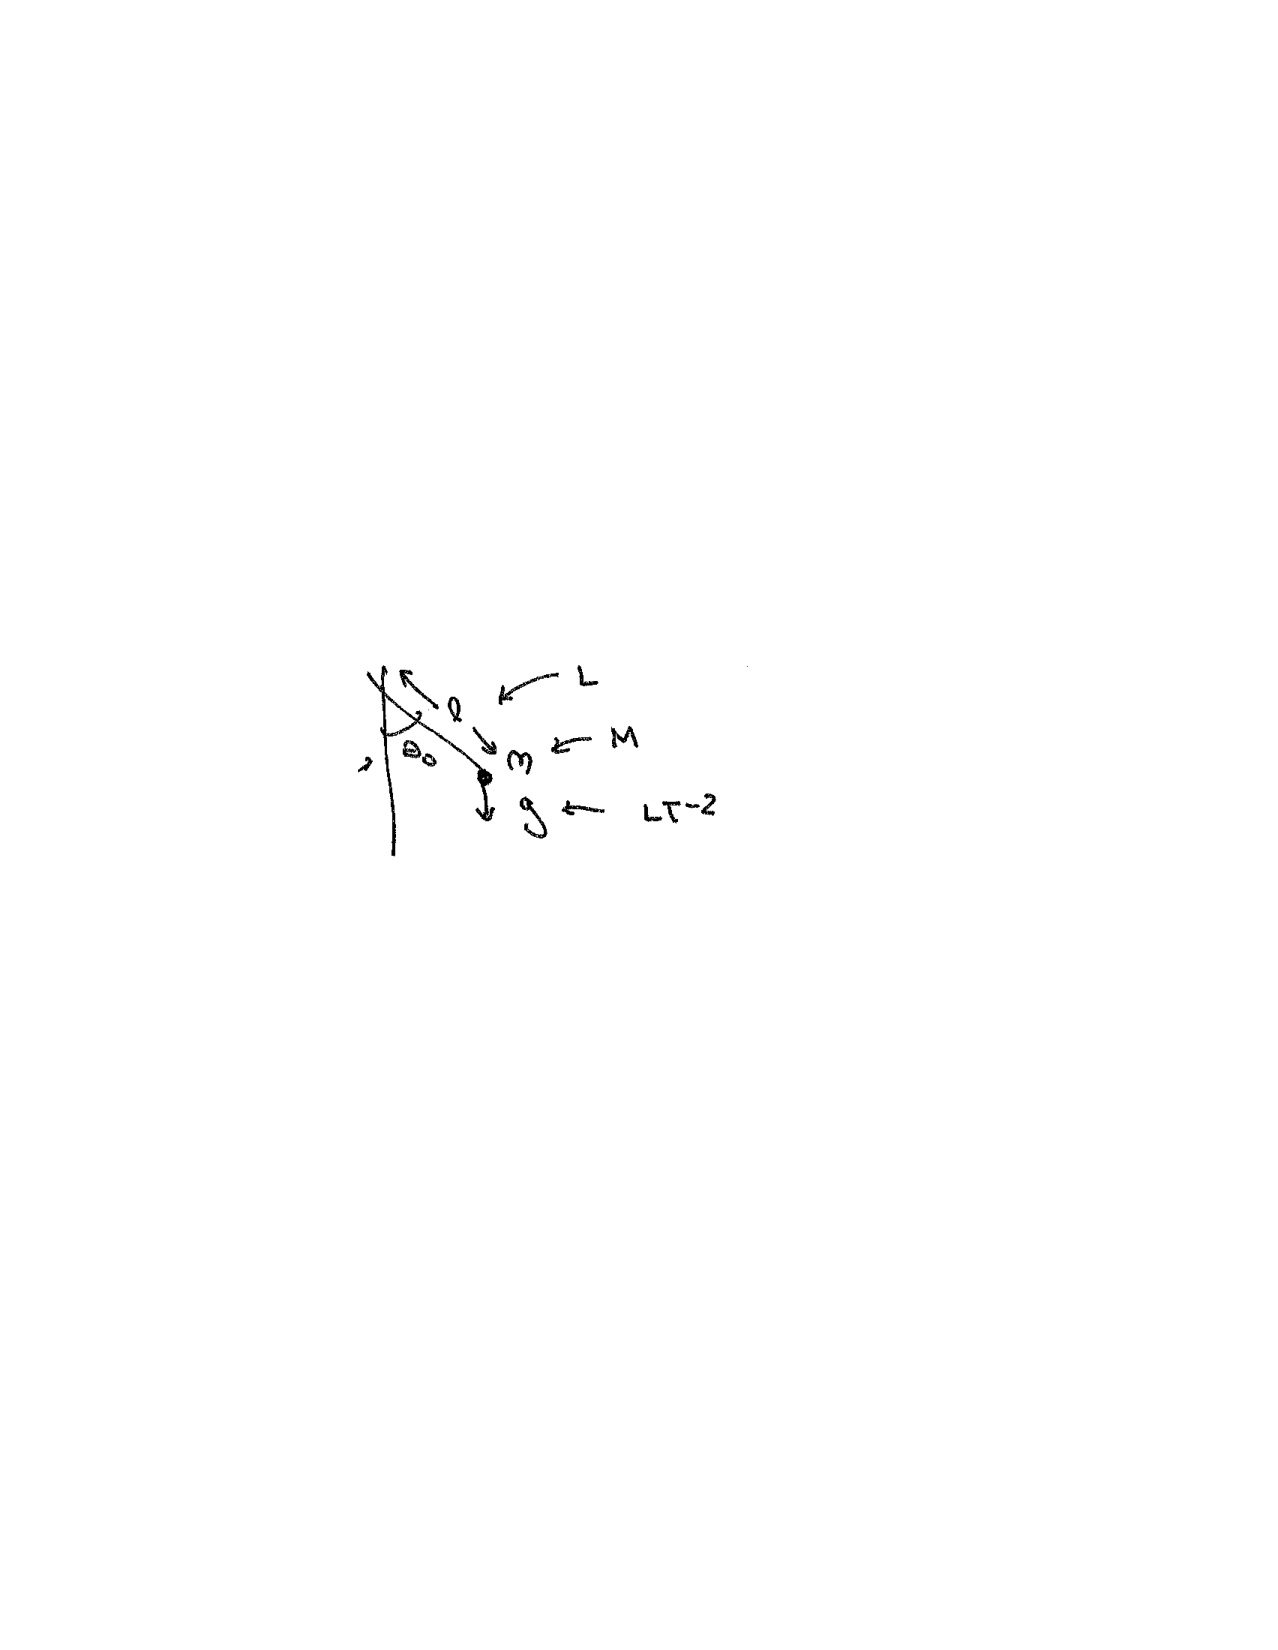
\includegraphics[width=.4\textwidth]{figures/lec01_pendulum.pdf}
\end{center}

From dimensional analysis, we know that the period has dimensions of time, $[\tau] = T$. The problem gives us a length $[\ell]=L$ and the gravitational acceleration, $[g]=LT^{-2}$. Note that $[\theta_0] = 1$ is dimensionless. This means that the only way to form a quantity with dimensions of time is to use $g^{-1/2}$. This leaves us with a leftover $L^{-1/2}$, which we can fix by inserting a square root of $\ell$:
\begin{align}
  \tau \sim g^{-1/2} \ell^{1/2} \ .
\end{align}
If we wanted to be fancy, we can make this an equal sign by writing a function of the other dimensionless quantities in the problem:
\begin{align}
  \tau = f(\theta_0) \sqrt{\frac{\ell}{g}} \ .
\end{align}

\subsection{Scaling}

A large part of physics has to do with scaling relations. Here’s a somewhat contrived example of how this works. Suppose you have some static, central potential $U(\vec r)$. Maybe it’s some planet orbiting a star. 

\begin{center}
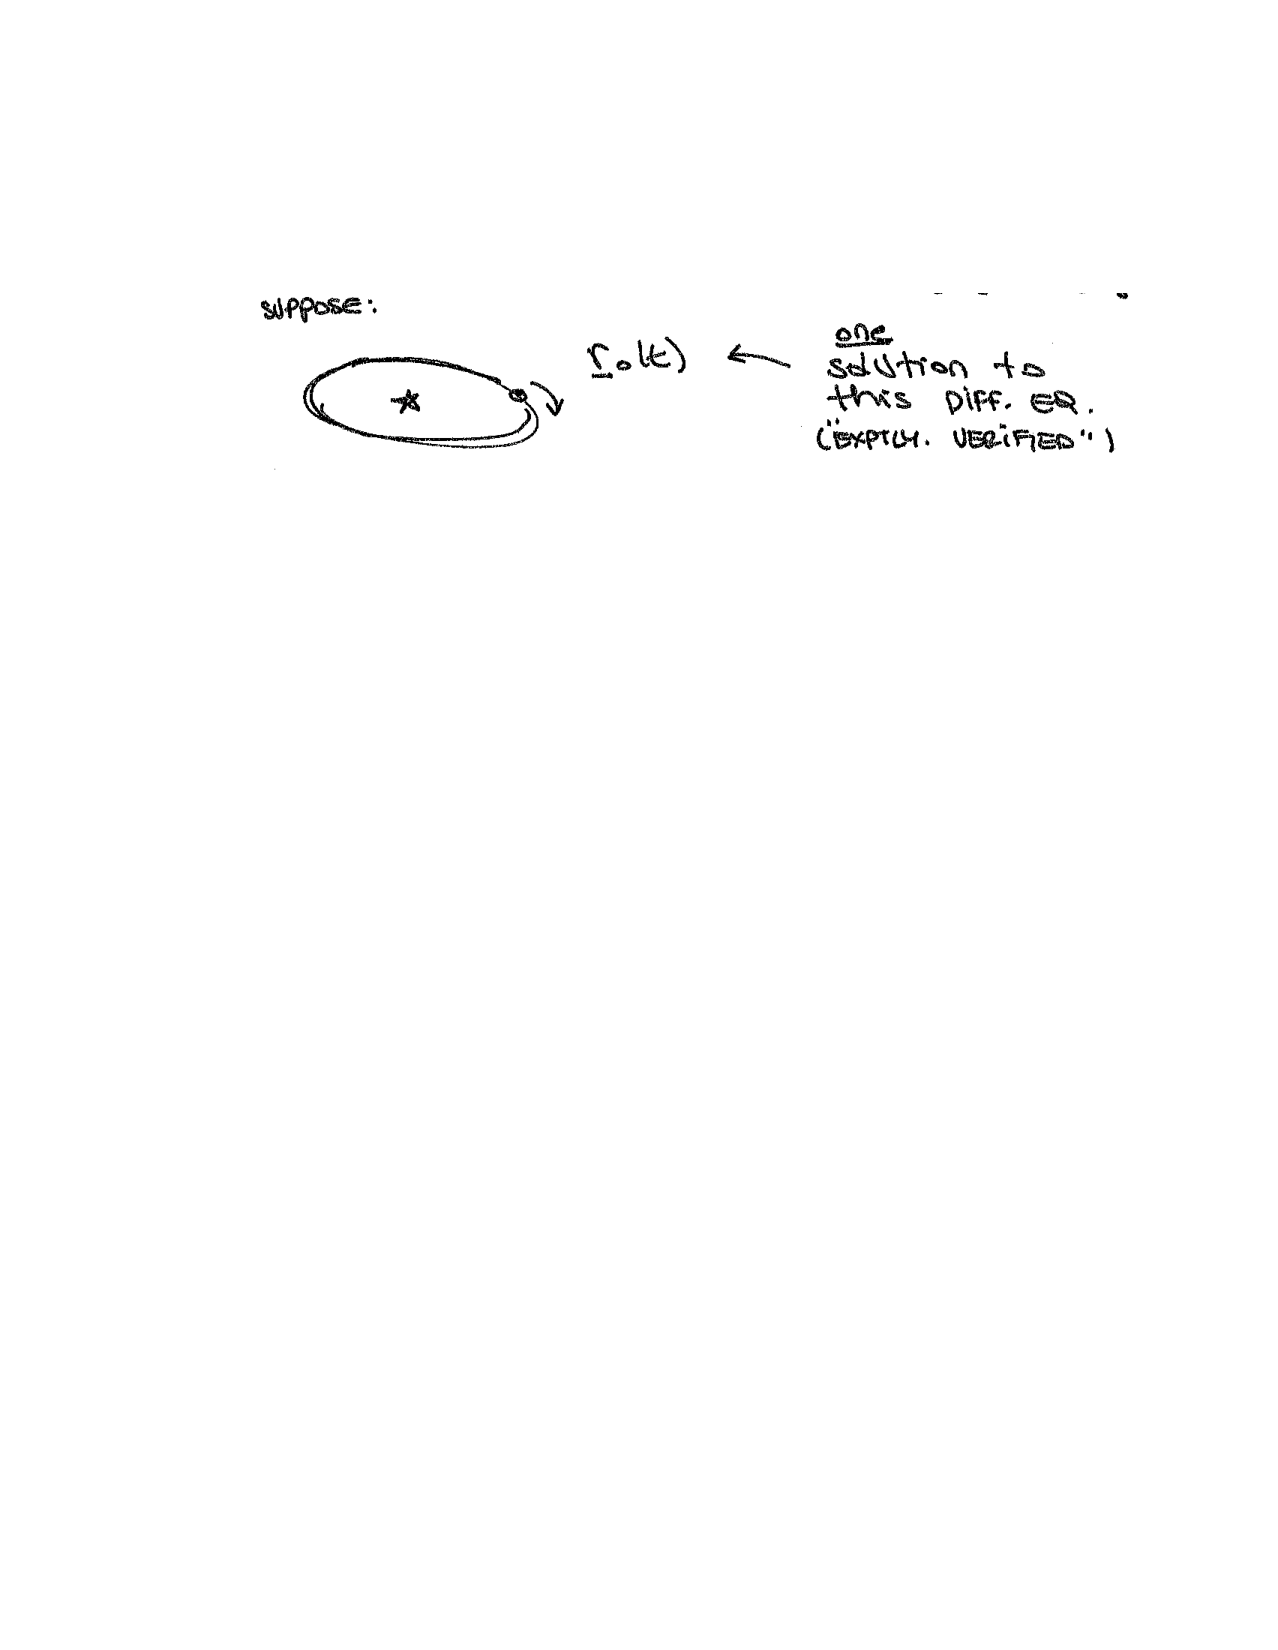
\includegraphics[width=.7\textwidth]{figures/lec01_orbit.pdf}
\end{center}

The force law gives:
\begin{align}
  m 
  \ddot{\vec{r}} = - \frac{\partial U}{\partial\vec{r}} \ .
\end{align}
Suppose we are given a solution, $\vec r_0(t)$. Perhaps this is a trajectory that is experimentally verified. Dimensional analysis gives a way to scale this solution into other solutions. For example, let us scale time by defining a new variable $t'$:
\begin{align}
  t \equiv \alpha t' \ .
\end{align}
If the potential is static, then only the left-hand side of the force law changes. Even though the right-hand side formally has dimensions of time $\sim T^{-2}$, it does not transform because those units are carried in a constant, perhaps $G_N$, not a $(d/dt)^2$ like the left-hand side. The left-hand side of the force law gives:
\begin{align}
  m\left(\frac{d}{dt}\right)^2 \vec r_0(t) 
  &=
  m\alpha^{-2} \left(\frac{d}{dt'}\right)^2 \vec r_0(\alpha t') \ .
\end{align}
This begs us to define a new mass $m' = m\alpha^{-2}$. We thus have
\begin{align}
   m'\ddot{\vec{r}}(\alpha t')
  = - \frac{\partial U}{\partial\vec{r}} \ .
\end{align}
What this tells us is that $\vec r_1(t') = r_0(\alpha t')$ is a solution in the same potential that traces the same trajectory but at $\alpha$ times the speed and with mass $m'$. For example, if $\alpha = 2$, then $\vec r_1(t)$ traces the same trajectory at double the velocity with one fourth of the mass. 

\subsection{Error Estimates}

This section is based on a lovely \emph{American Journal of Physics} article by Craig Bohren.\footnote{\url{https://doi.org/10.1119/1.1574042}} Let’s go back to another high school physics problem. 

\begin{center}
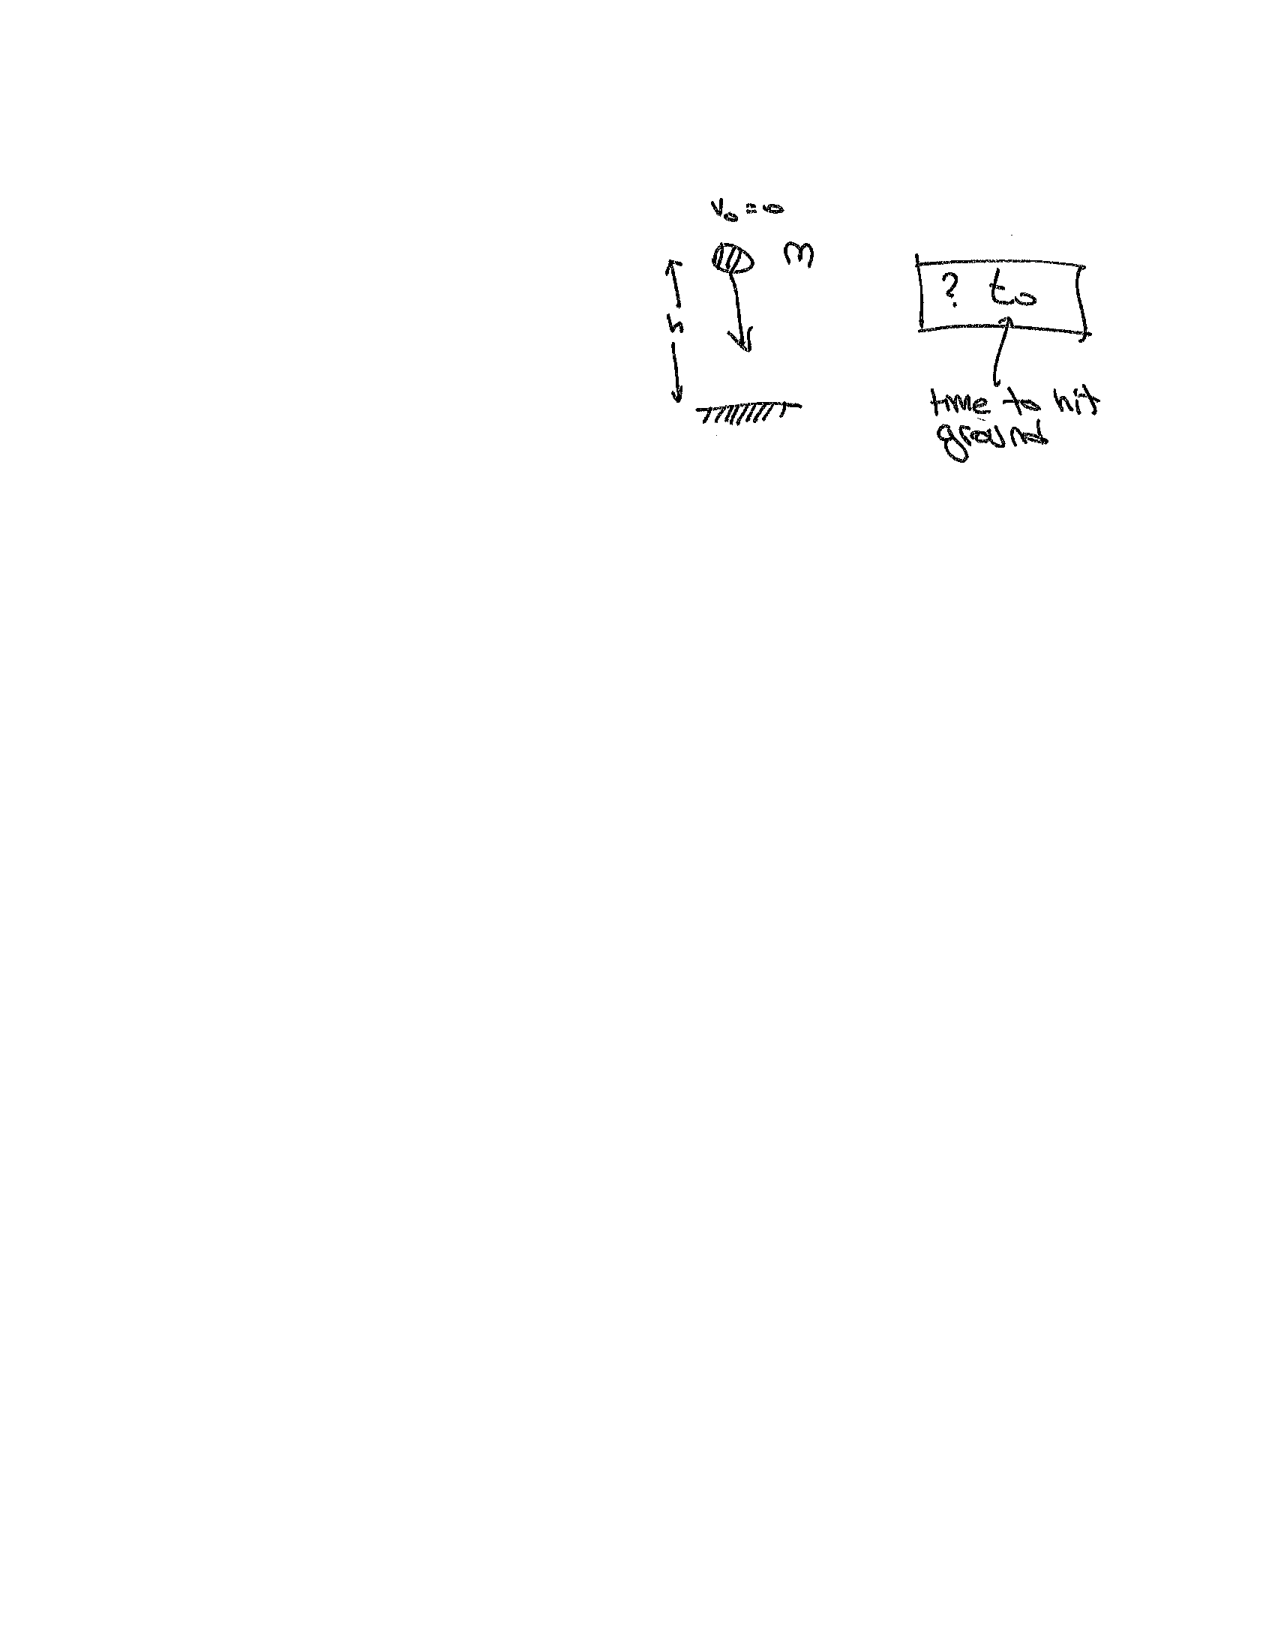
\includegraphics[width=.4\textwidth]{figures/lec01_drop.pdf}
\end{center}

Suppose you drop a mass $m$ from height $h$ that is initially at rest. How long before this hits the ground? You can integrate the force equation to get
\begin{align}
  t_0 = \sqrt{\frac{2h}{g}} \ .
\end{align}
This is the \emph{exact} answer \emph{within our model} of the system. The model made several assumptions. The mass is a point mass, the gravitational acceleration is constant at all positions, there is no air resistance, etc. In fact, we \emph{know} that if we do an experiment, our result will almost certainly \emph{not} be $t_0$. All we know is that $t_0$ is probably a good approximation of what the actual answer is.

\emph{How good of an approximation is it?}

One way to do this is to do the next-to-leading order (`NLO‘) calculation, taking into account a more realistic (and hence more complicated) model and then compare to $t_0$. But this is stupid. Why do we need to do a \emph{hard} calculation to justify doing an \emph{easy} one? If we’re going to do the hard calculation anyway, what’s the point of ever doing the easy one?

What we really want is an error estimate. The error is
\begin{align}
  \epsilon &= \frac{t_1 - t_0}{t_0} \ .
\end{align}
This is a dimensionless quantity that determines how far off $t_0$ is from a more realistic calculation, $t_1$. Ideally we don’t actually have to do work to get $t_1$. 

Let’s assume that we’re not completely nuts and that we’re in a regime where the error is small\footnote{Note the error has to be dimensionless in order for us to be able to call it `small,` otherwise it begs the question of `small with respect to what?`}. Then the error is a function of some dimensionless parameters, $\xi$, in the system. We define these $\xi$ so that as $\xi \to 0$, $\epsilon(\xi) \to 0$. In other words, the approximation gets better as the $\xi$ are made smaller. By Taylor expansion:
\begin{align}
  \epsilon(\xi) = \epsilon(0) + f'(0) \xi + \mathcal O(\xi^2) \ .
\end{align}
By assumption  $\epsilon(0) = 0$ and $\mathcal O(\xi^2)$ is  small. We can then make a reasonable assumption that the dimensionless value $f'(0)$  is $\mathcal O(1)$. This tells us that the error goes like $\epsilon(\xi) \sim \xi$.

Here’s how it works in practice. One effect that we miss in our toy calculation of $t_0$ is that the earth is round with radius $R$. This means that assuming a constant $g$ is an approximation. We have two choices for a dimensionless parameter $\xi$:
\begin{align}
  \xi &= \frac{h}{R}
  &\text{or}&&
  \xi &= \frac{R}{h} \ .
\end{align}
There is an obvious choice: $\xi = h/R$, because we know that as $h$ is made smaller (drop the ball closer to the ground) or $R$ becomes bigger (larger radius of Earth) then the constant $g$ approximation gets better. We thus expect that the corrections from the position-dependence of $g$ go like $\mathcal O(h/R)$.
 
% Exercise: check by explicit calculation, 2017 lec 1


\subsection{Bonus: Allometry}

There’s a fun topic called \textbf{allometry}. This is basically dimensional analysis applied to biology. A typical example is to consider two people who have roughly the same shape but different characteristic lengths, $\ell$ and $L$:

\begin{center}
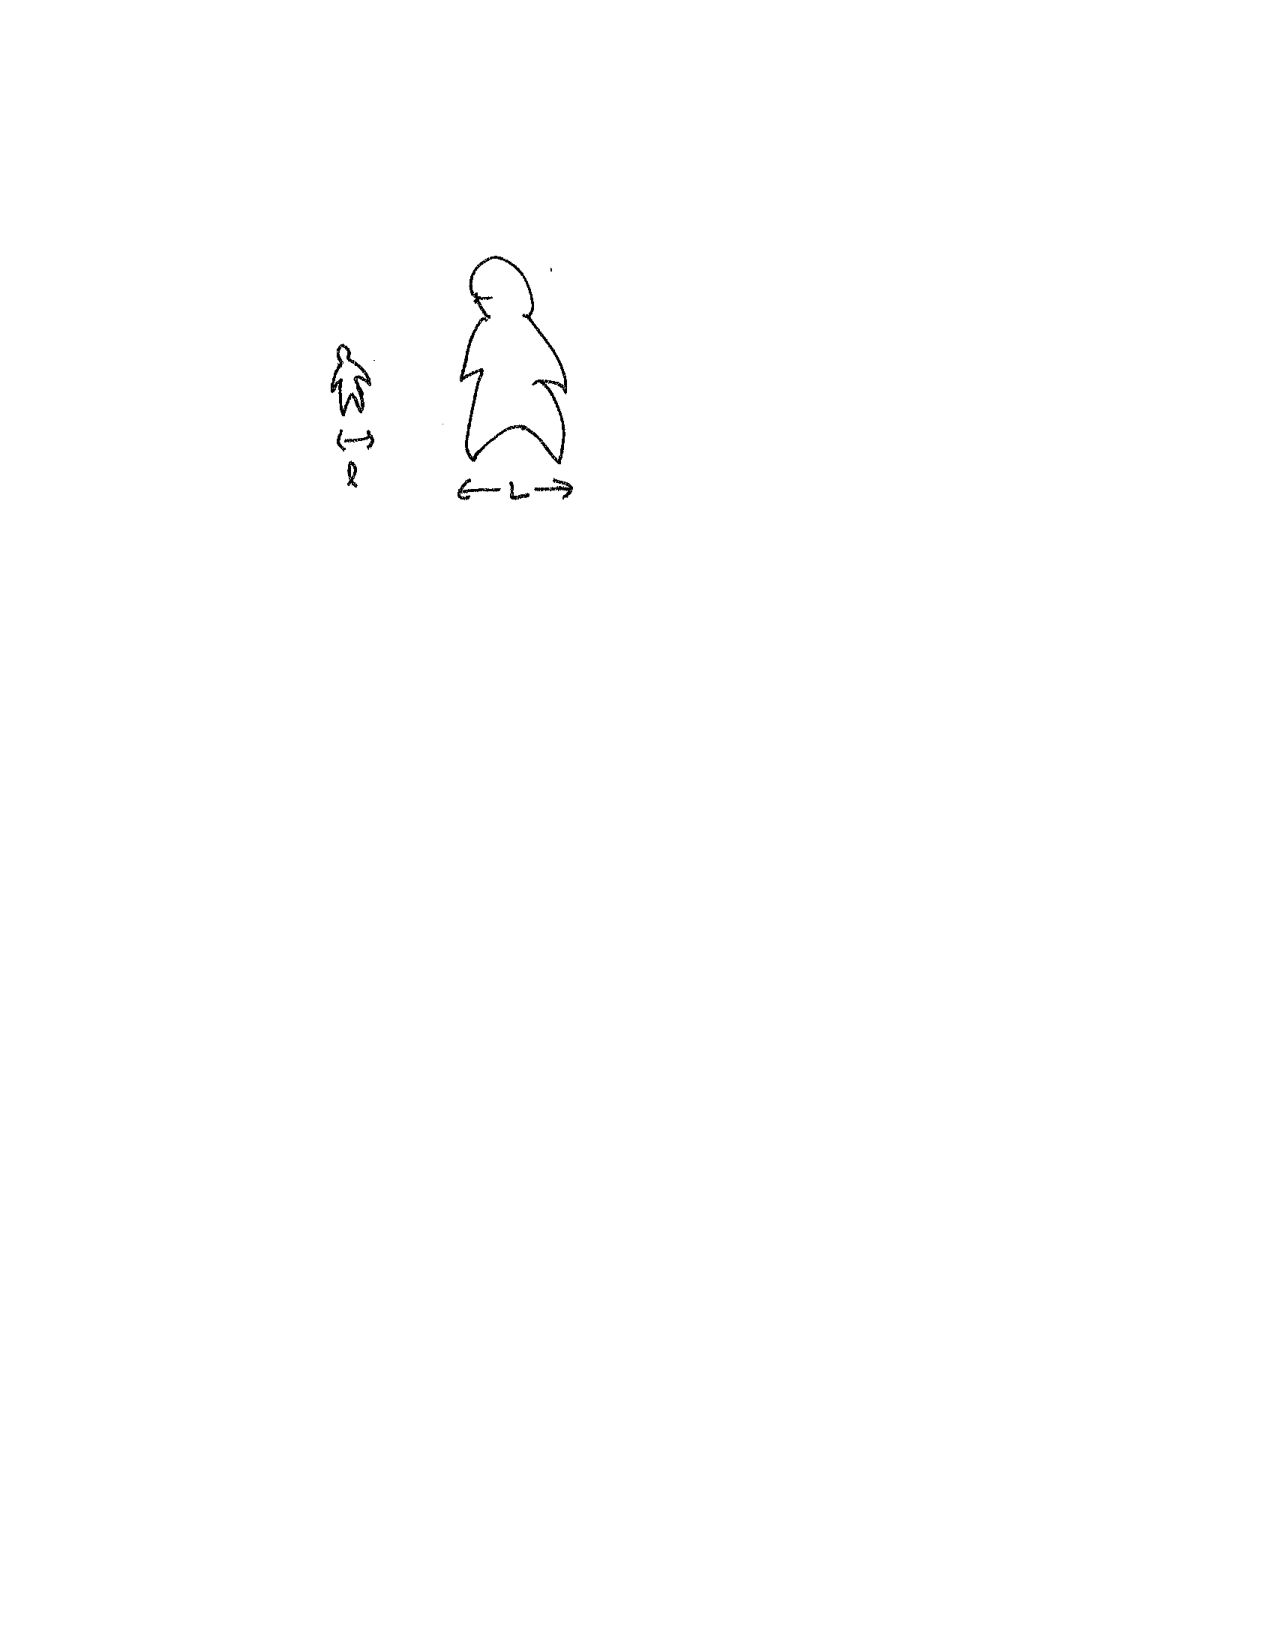
\includegraphics[width=.4\textwidth]{figures/lec01_allometry.pdf}
\end{center}

If both people exercised at the same rate, which one loses more absolute weight? By how much? Let’s assume that weight loss is primarily from the conversion of organic molecules into carbon dioxide. 







\section{Linear Algebra Review}

The usual joke is that we all know linear algebra from kindergarten, at which point students roll their eyes. As physicists, linear algebra is part of our DNA from the vector calculus of our first electrodynamics course to quantum mechanics. Why, then should we patronize ourselves with yet another review of linear algebra?

Our goal is to understand Green’s functions as \emph{matrix inverses}. They are the inverse of matrices that represent the differential operator of the differential equation that we’d like to solve. These matrices act on a space of functions. Our goal is to use linear algebra to build an intuition for Green’s functions. We start with reminders of facts from your mathematical `childhood,` but throughout it all we would like to keep the following in mind:
\begin{align}
  \text{function space} &= \infty\text{-dimensional vector space} \ .
\end{align}

\subsection{The basics}

A \textbf{linear transformation} $A$ acts on a vector $\vec{v}$ as $A\vec{v}$. 
This transformation satisfies
\begin{align}
  A(\alpha \vec{v}+ \beta \vec{w}) = \alpha A\vec{v} + \beta A\vec{w} \ .
\end{align}
Here $\alpha$ and $\beta$ are numbers.
%
This is conventionally matrix multiplication. The result is also a vector. One way that we like to think about vectors is as columns of elements:
\begin{align}
  \begin{pmatrix}
    v^{1} \\ v^{2} \\ \vdots \\ v^{N}
  \end{pmatrix} \ ,
\end{align}
where $N$ is the \textbf{dimension} of the vector space. Our notation is that $v^i$ refers to the $i^\text{th}$ component of $\vec{v}$. Sometimes---as physicists---we refer to $v^i$ as the vector itself, which is a slight abuse of notation that occasionally causes confusion.

Matrix multiplication may actually have been something you learned in grade school. Here’s how it works in two dimensions. A transformation that takes vectors into vectors takes the following form:
\begin{align}
  A &= 
  \begin{pmatrix}
   A^{1}_{\phantom{1}1} & A^{1}_{\phantom{1}2}
   \\
   A^{2}_{\phantom{1}1} & A^{2}_{\phantom{1}2}
  \end{pmatrix} \ .
\end{align}
We’re being fancy and using upper and lower indices. The significance is not pertinent at the moment, but practitioners of special relativity should nod with familiarity. If you’re squeamish about the indices, don’t worry: the elements of $A$ have two indices, the first one is written a little higher than the second one. This notation is neither mathematics nor physics, it’s a convention that we use for future convenience.

The action of $A$ on $\vec{v}$ is:
\begin{align}
  A\vec{v}
  =
  \begin{pmatrix}
    A^{1}_{\phantom{1}1} & A^{1}_{\phantom{1}2}
   \\
   A^{2}_{\phantom{2}1} & A^{2}_{\phantom{2}2}   
  \end{pmatrix} 
  \begin{pmatrix}
    v^1\\
    v^2
  \end{pmatrix}
  =
  \begin{pmatrix}
    A^1_{\phantom{1}1} v^1 + A^1_{\phantom{1}2}v^2\\
    A^2_{\phantom{2}1} v^2 + A^2_{\phantom{2}2}v^2
  \end{pmatrix} \ .
\end{align}
Look at this carefully. The components of the new vector $(A \vec{v})^i$ are sums. In each term, the second/lower index of an $A$ element multiplies the component of $\vec{v}$ with the same index. The first/upper index of $A$ tells you whether that term should is in $(A \vec{v})^1$ or $(A \vec{v})^2$. 

A generic component of $(A\vec{V})$ is
\begin{align}
  (A\vec{v})^i = \sum_j A^i_{\phantom{i}j} v^j
  = A^i_{\phantom{i}j} v^j \quad \text{(Einstein convention)}
   \ .
\end{align}
On the right-hand side we use Einstein notation: \emph{we implicitly sum over repeated upper/lower indices}. We will use this notation from now on.
%
If you are at all in doubt about this, please work out the $2\times 2$ case carefully and compare to the succinct notation above. 


If $A$ and $B$ are linear transformations, then $A+B$ is a linear transformation. The components of $A+B$ are simply the piecewise sum of the corresponding components of $A$ and $B$:
\begin{align}
  (A+B)^i_{\phantom i j} = A^i_{\phantom i j} + B ^i_{\phantom i j} \ .
\end{align}

\subsection{Linear Transformations and Vector Space}

Let’s be a little more pedantic. We should \emph{not} think of a vector $\vec{v}$ as some `column of numbers.' The power of this formalism is that a vector space is abstract. The layer of abstraction is encoded in the basis vectors, which we write as $\vec{e}_{(i)}$. For a space of dimension $N$, there are $N$ such vectors indexed by the subscript. Let us more formally write the vector $\vec{v}$ as
\begin{align}
  \vec{v} = 
  v^1 \vec{e}_{(1)}
  +
  v^2 \vec{e}_{(2)} + \cdots
  = v^i \vec{e}_{(i)} \ .
\end{align}
These basis vectors may be unit vectors in space. They may be represented by unit column vectors, e.g.
\begin{align}
  \vec{e}_{(1)}
  &= 
  \begin{pmatrix}
  1 \\ 0 \\ 0
  \end{pmatrix}
  &
    \vec{e}_{(2)}
  &= 
  \begin{pmatrix}
  0 \\ 1 \\ 0
  \end{pmatrix}
  &
  \cdots \ .
\end{align}
But these may be more general objects. For example, you can specify a color of light by specifying the red/green/blue content. We could have $\vec{e}_{(1)}$ be a unit amount of red light, $\vec{e}_{(2)}$ be a unit amount of green light, and $\vec{e}_{(3)}$ be a unit amount of blue light. Then a 3-vector $\vec{v}$ would correspond to light of a particular color. This color space is a vector space.




\subsection{A funny vector space: histogram space}

Here’s a funny vector space that we’re going to use as a pedagogical crutch. Imagine histogram-space. The basis vectors are:

\begin{center}
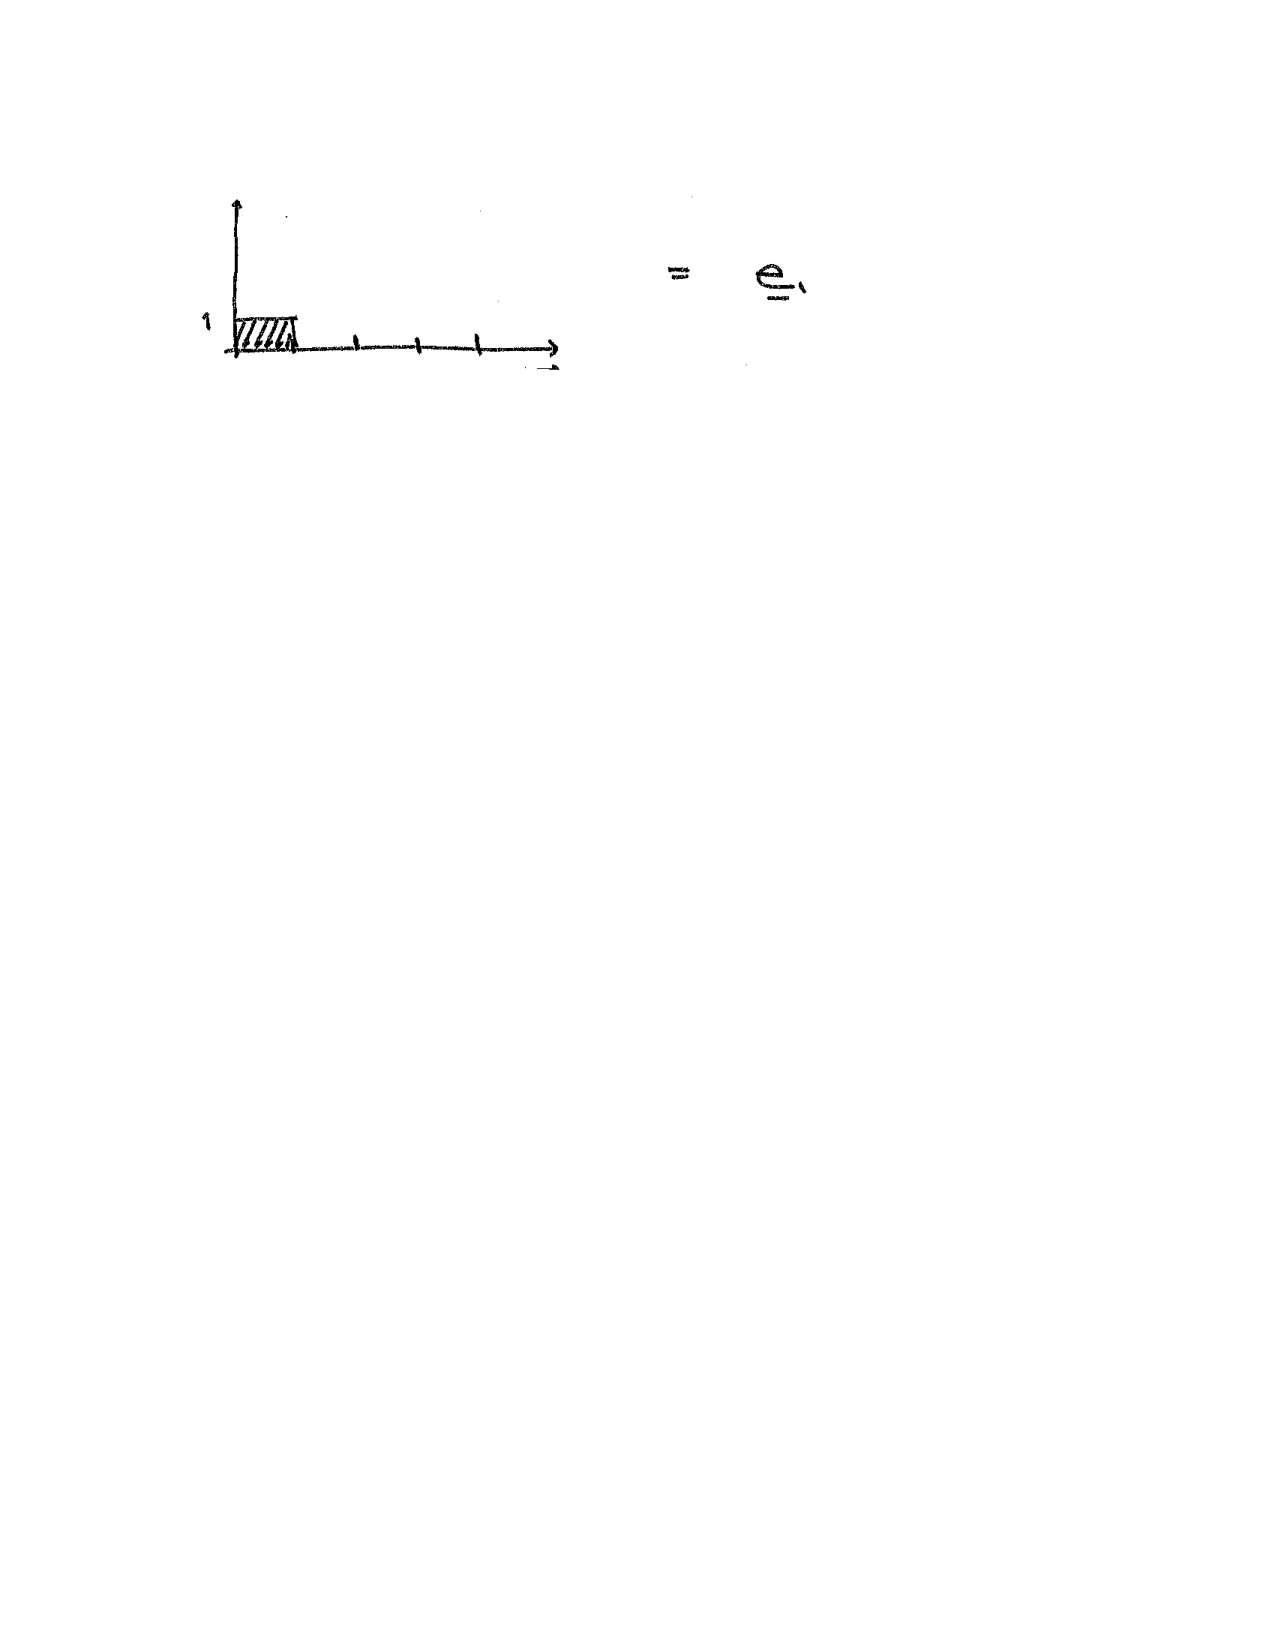
\includegraphics[width=.45\textwidth]{figures/lec02_e1.pdf}
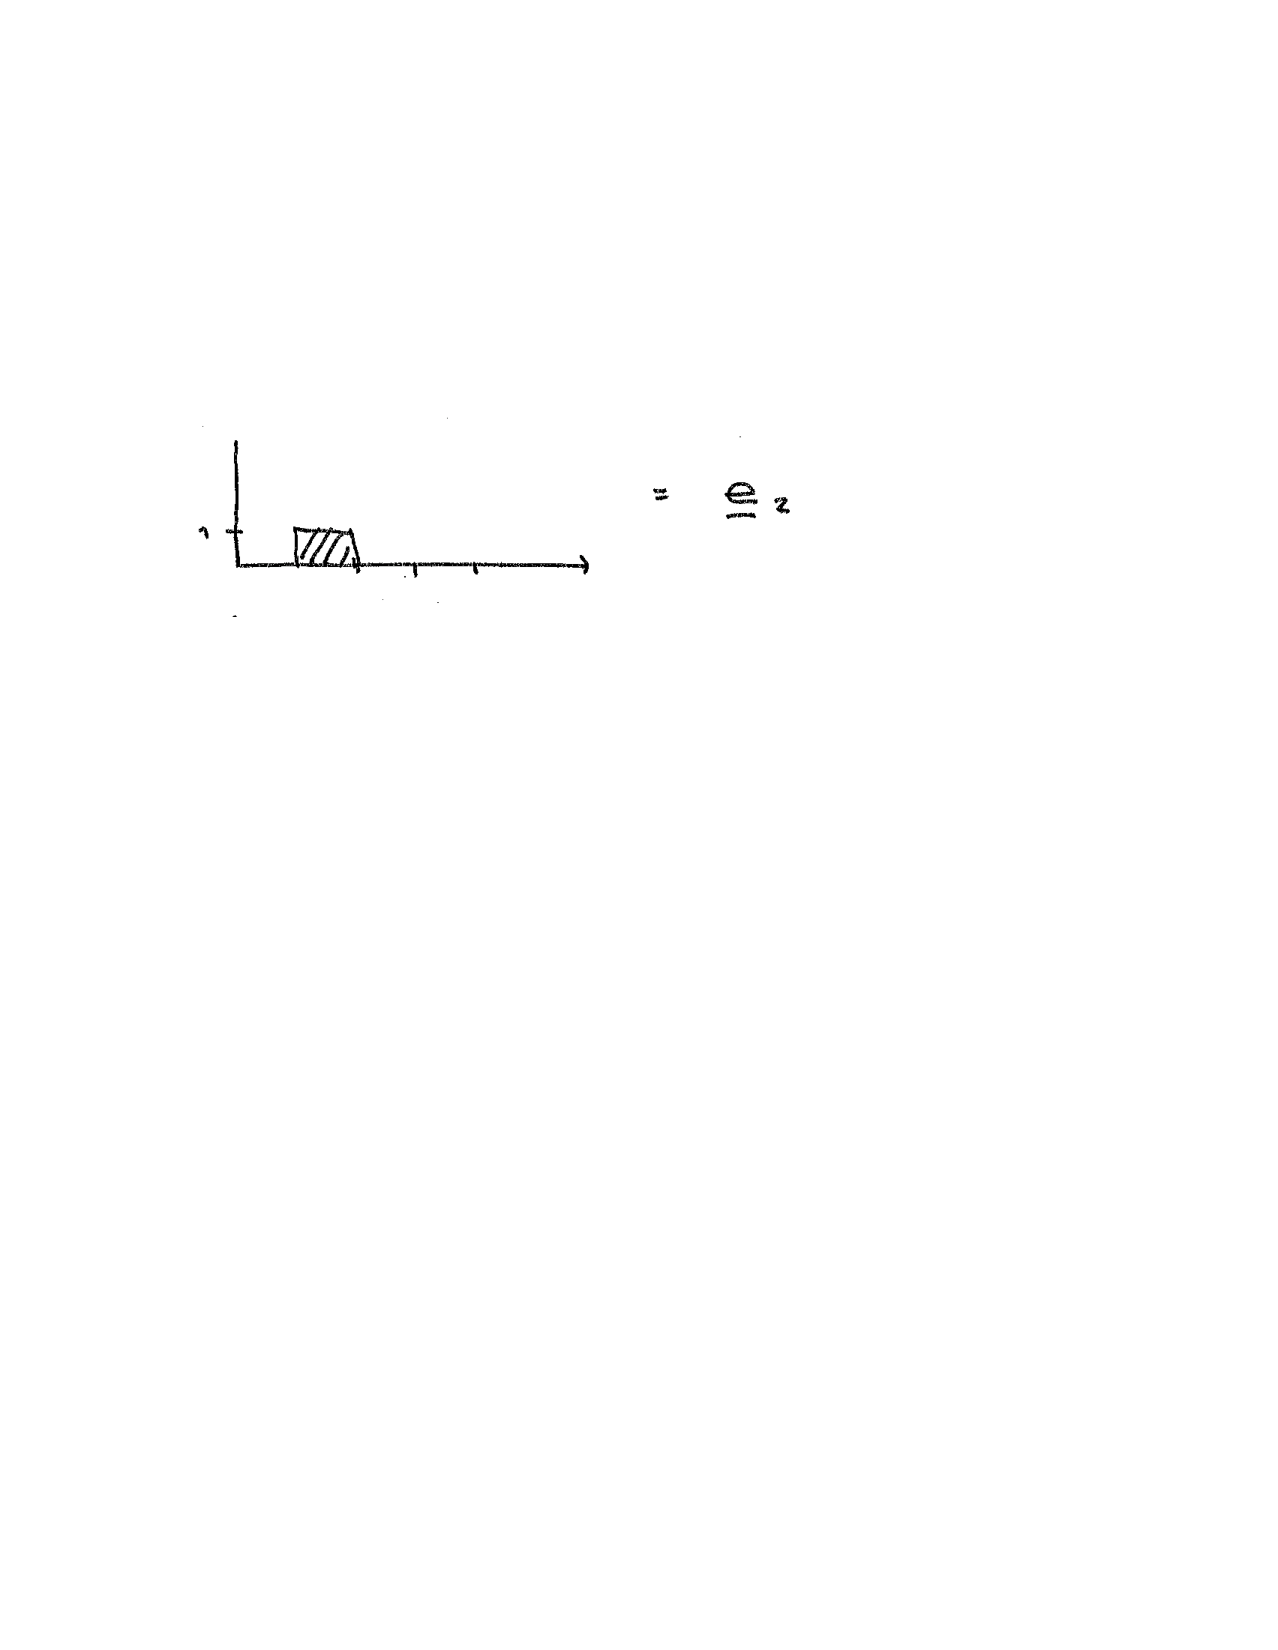
\includegraphics[width=.45\textwidth]{figures/lec02_e2.pdf}\\
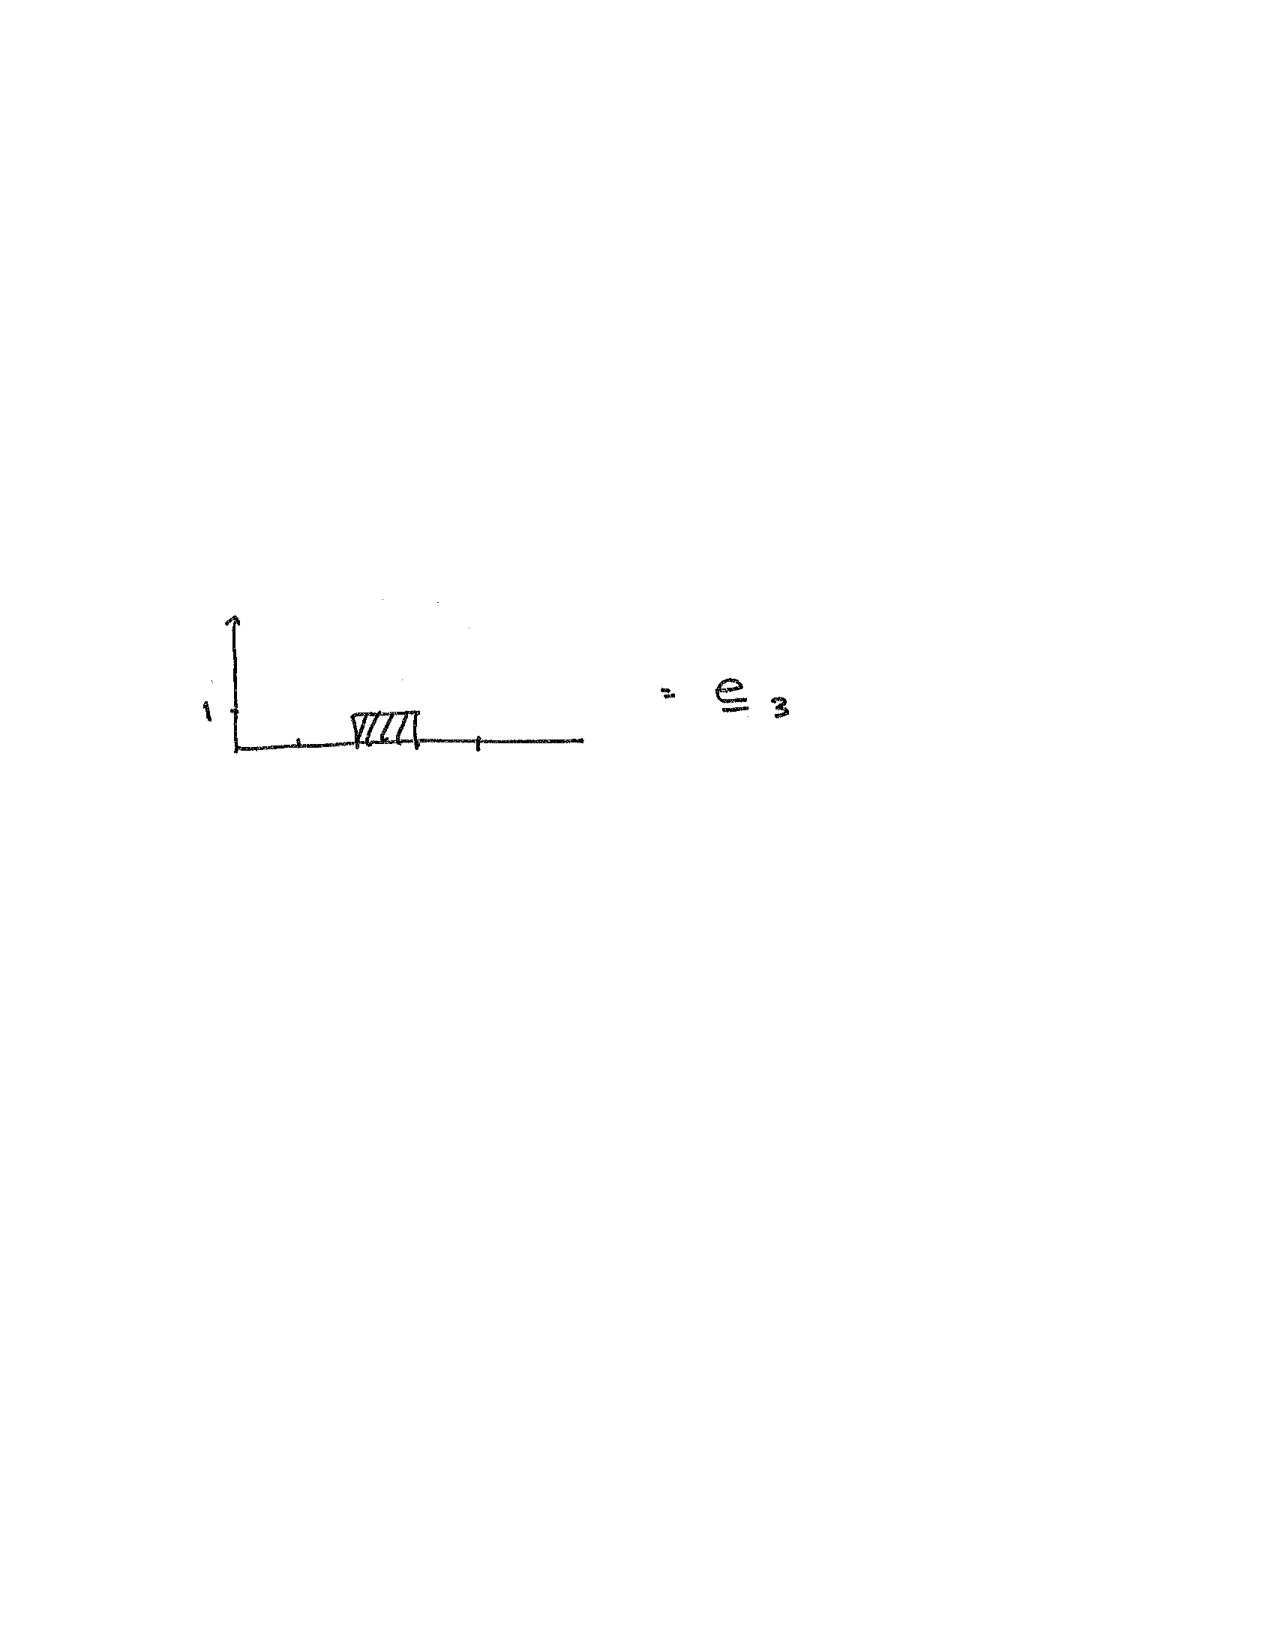
\includegraphics[width=.45\textwidth]{figures/lec02_e3.pdf}
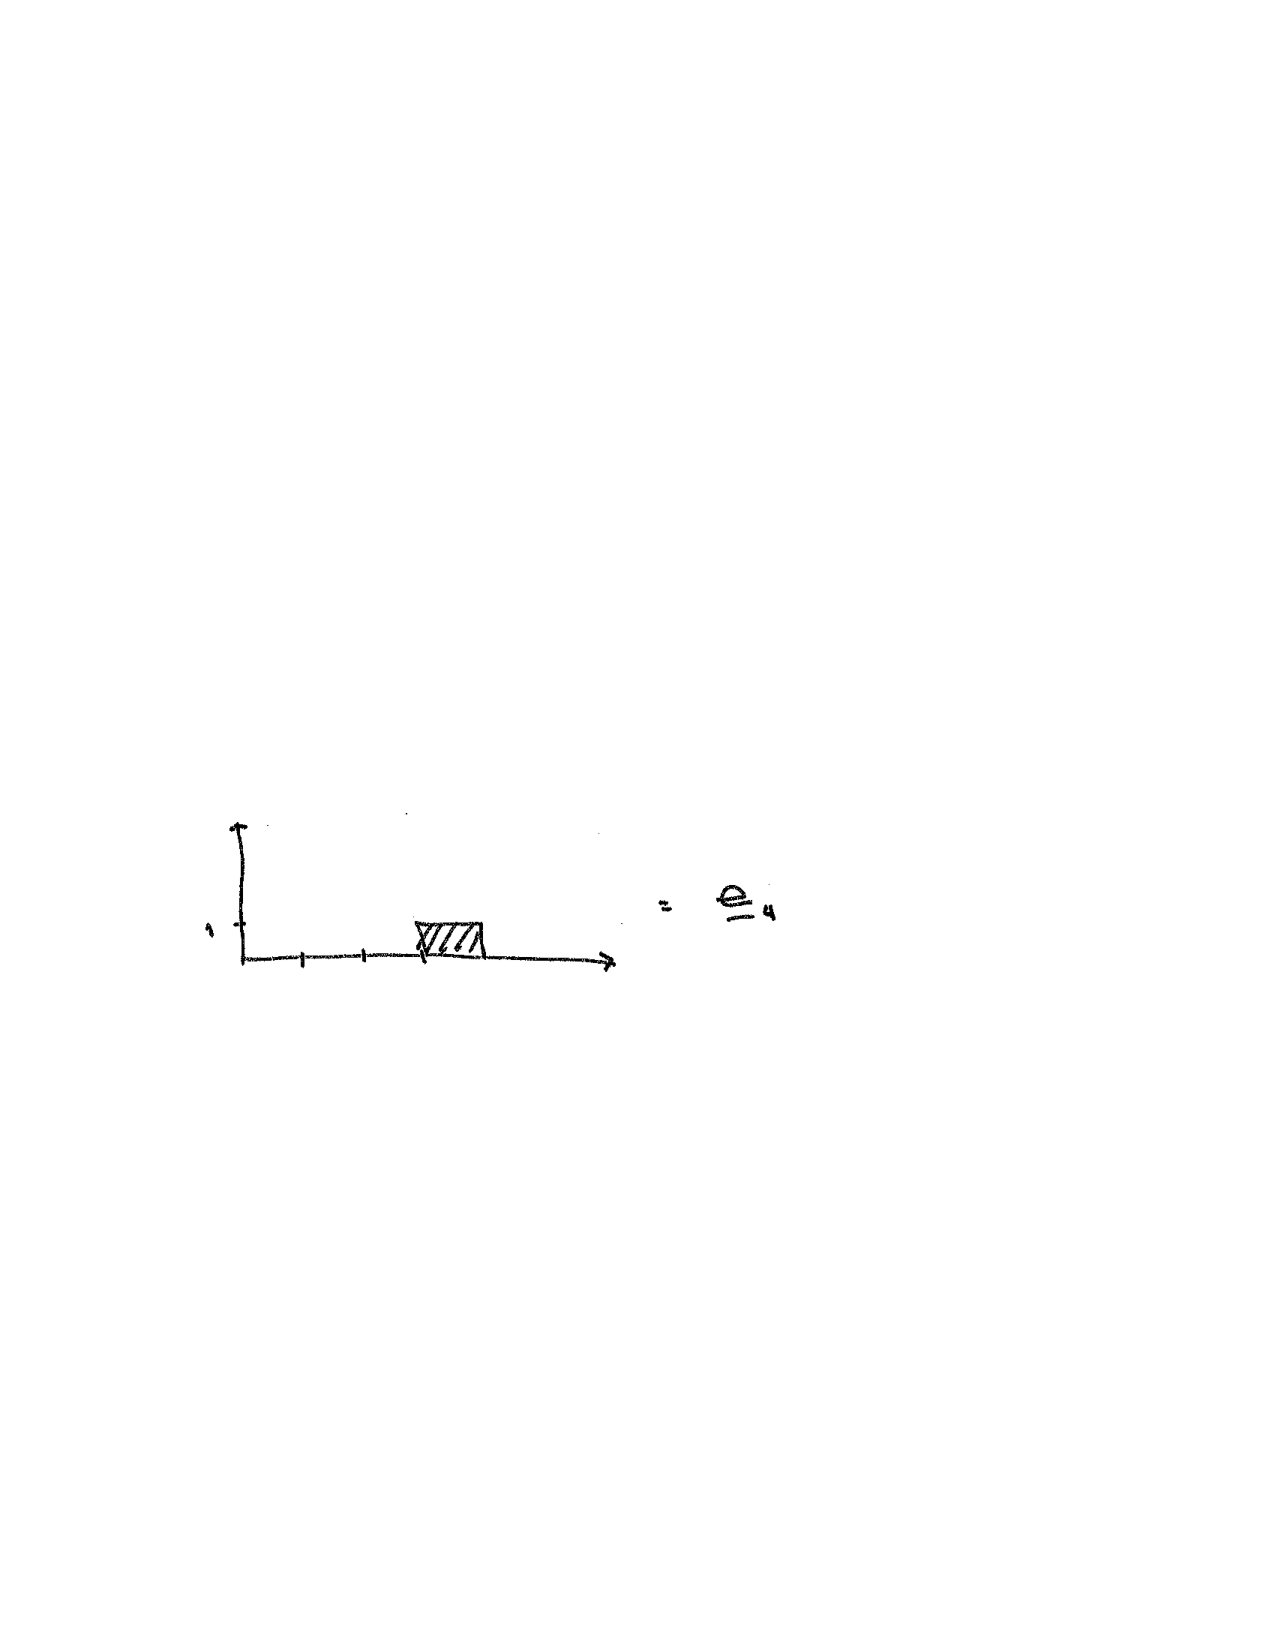
\includegraphics[width=.45\textwidth]{figures/lec02_e4.pdf}
\end{center}

This is a basis for a histogram over unit bins from $x=0$ to $x=4$. A vector in this space is, for example:

\begin{center}
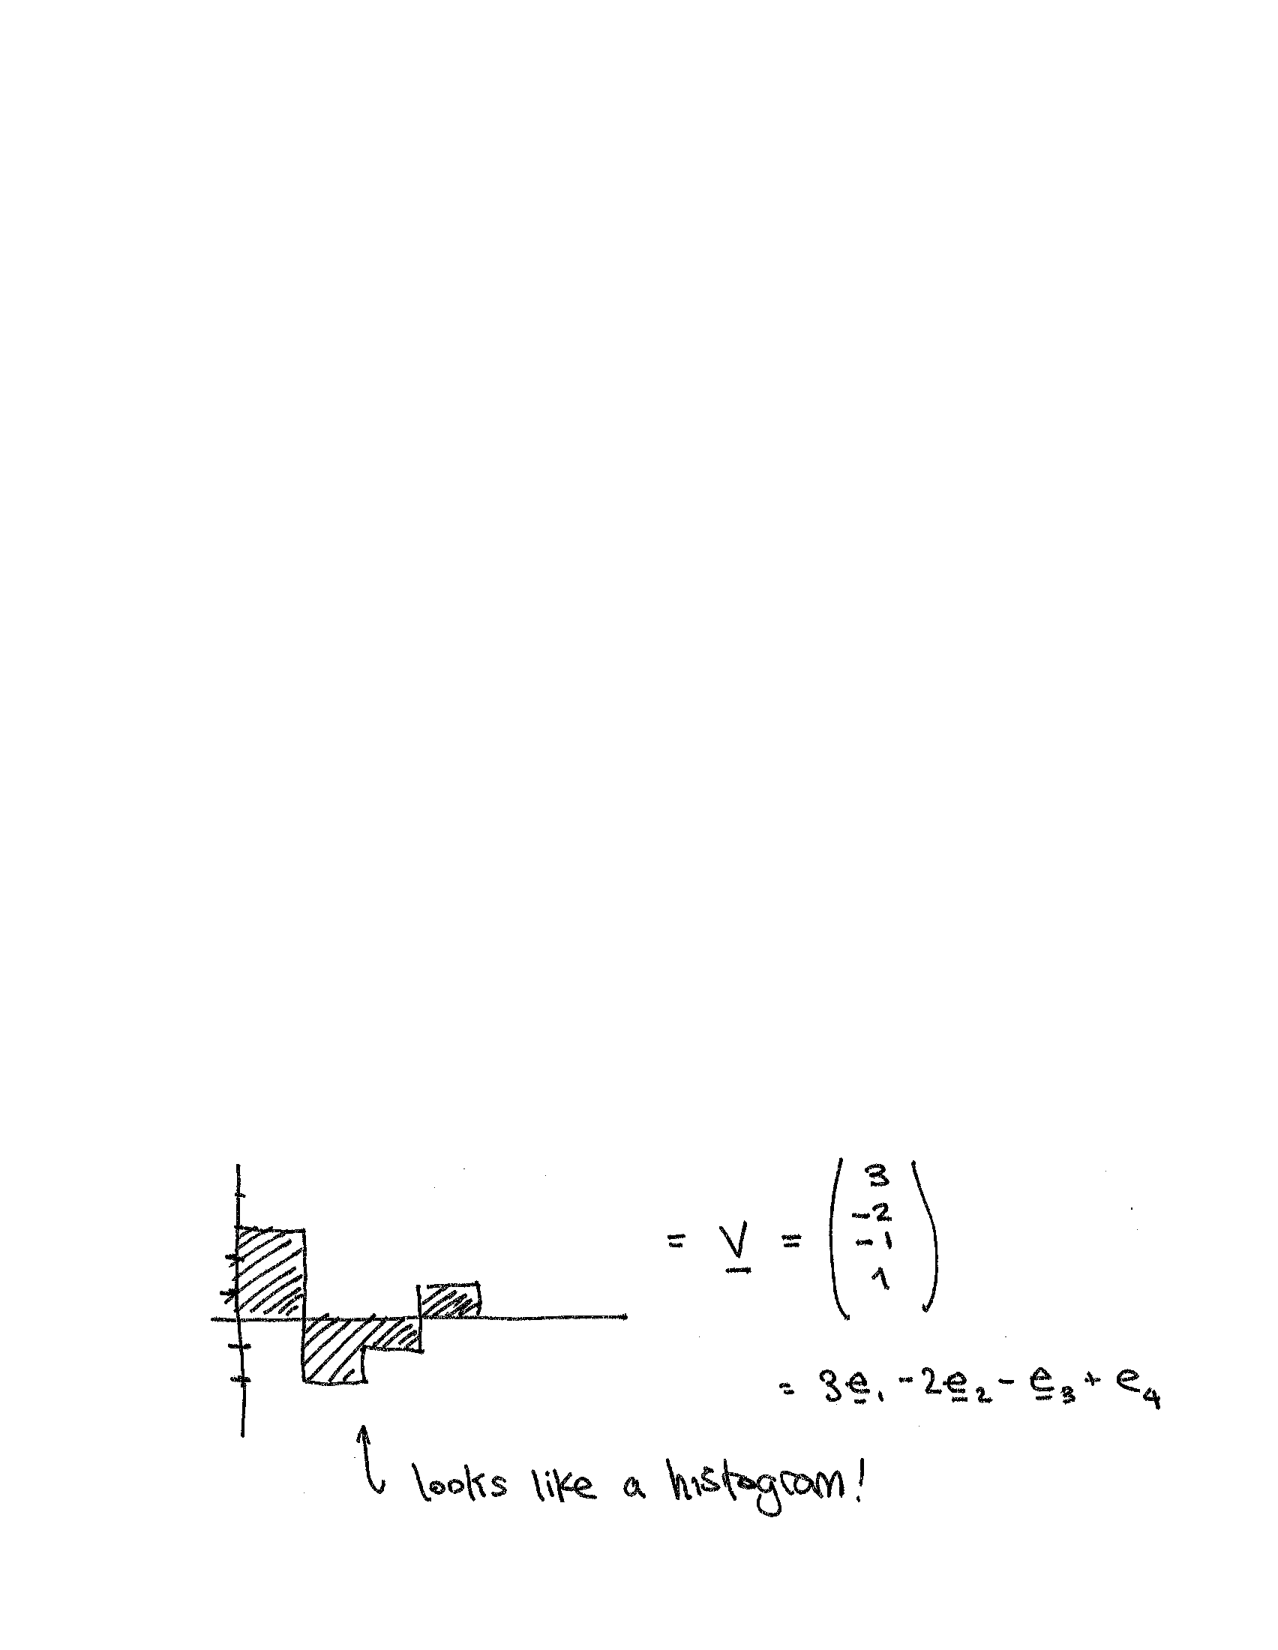
\includegraphics[width=.8\textwidth]{figures/lec02_hist.pdf}
\end{center}

We can perform a linear transformation $A$ on $\vec{v}$ which outputs another vector. Let’s say it’s this:


\begin{center}
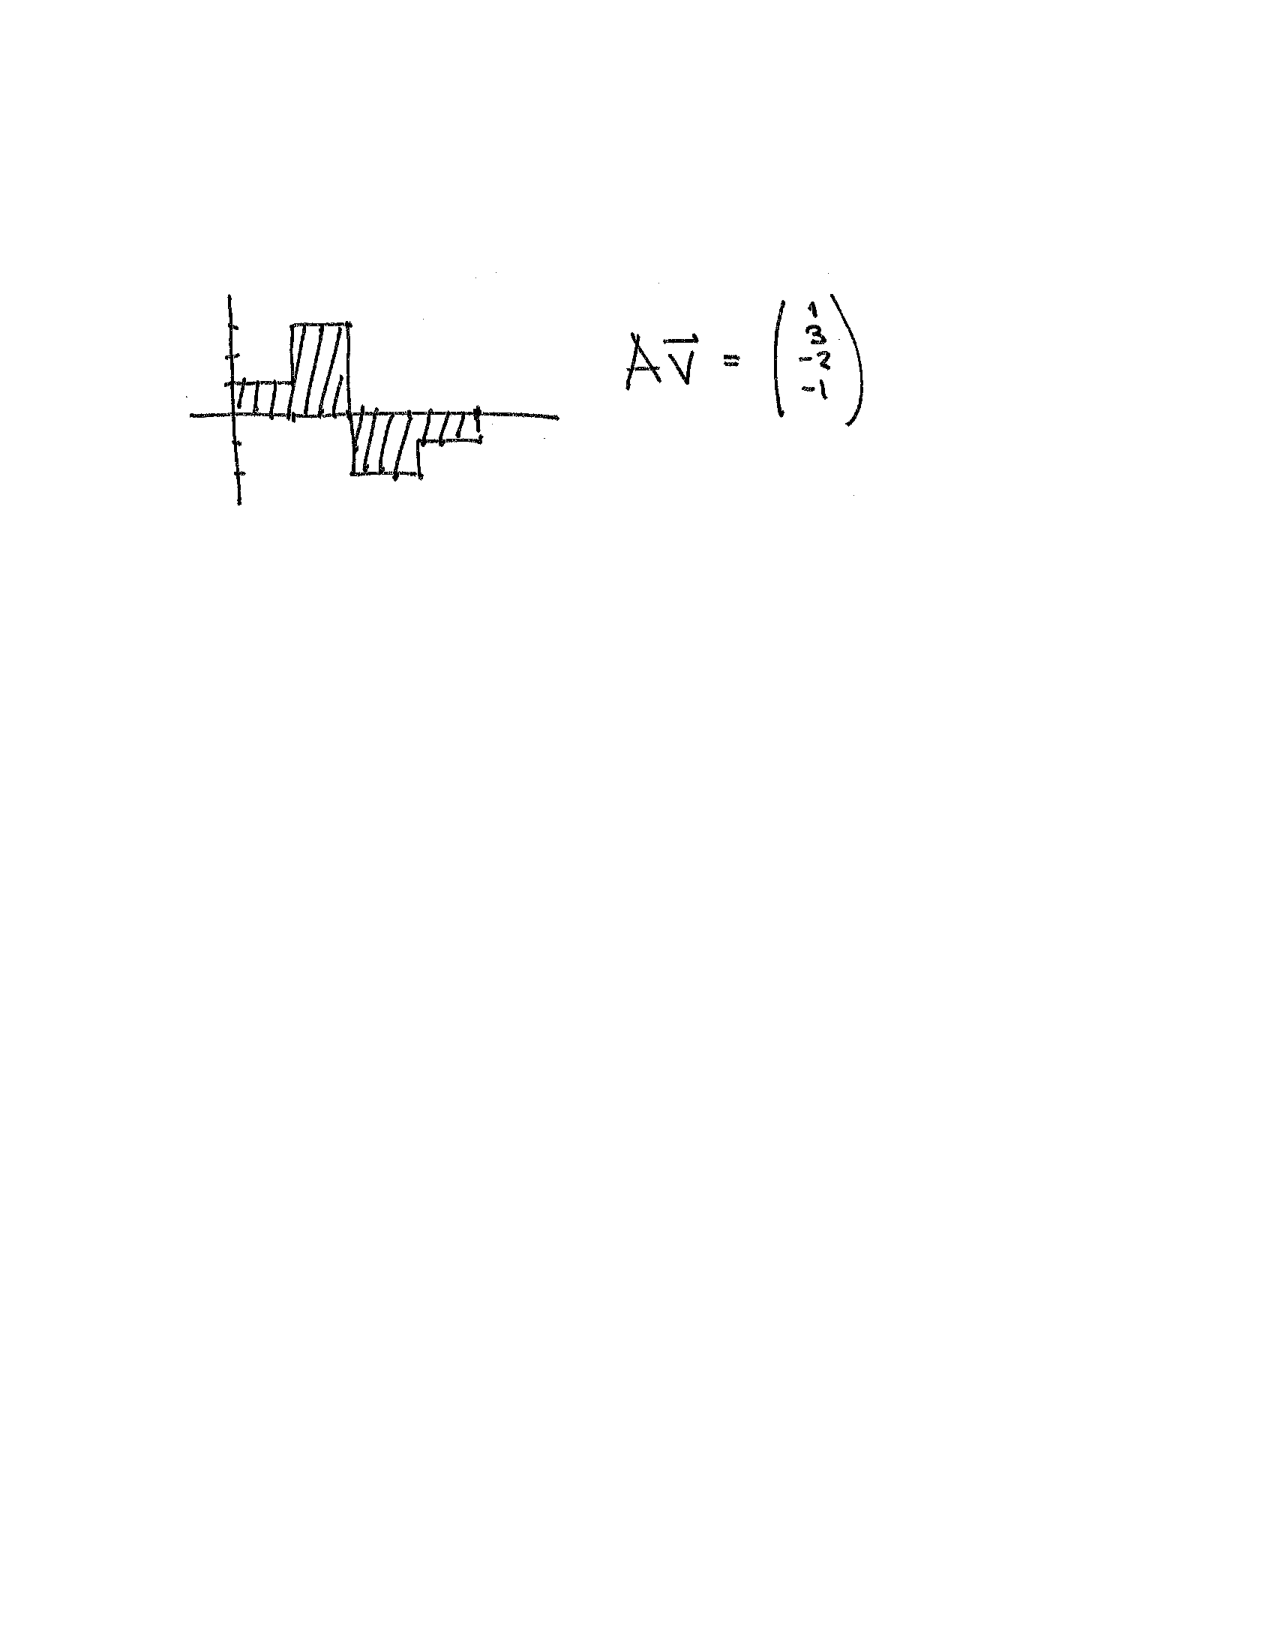
\includegraphics[width=.8\textwidth]{figures/lec02_hist2.pdf}
\end{center}

Sanity check: from this, can you derive what $A$ is? Answer: no. 

The power of this admittedly strange formalism is that we can think of these histograms as approximations of continuous functions:

\begin{center}
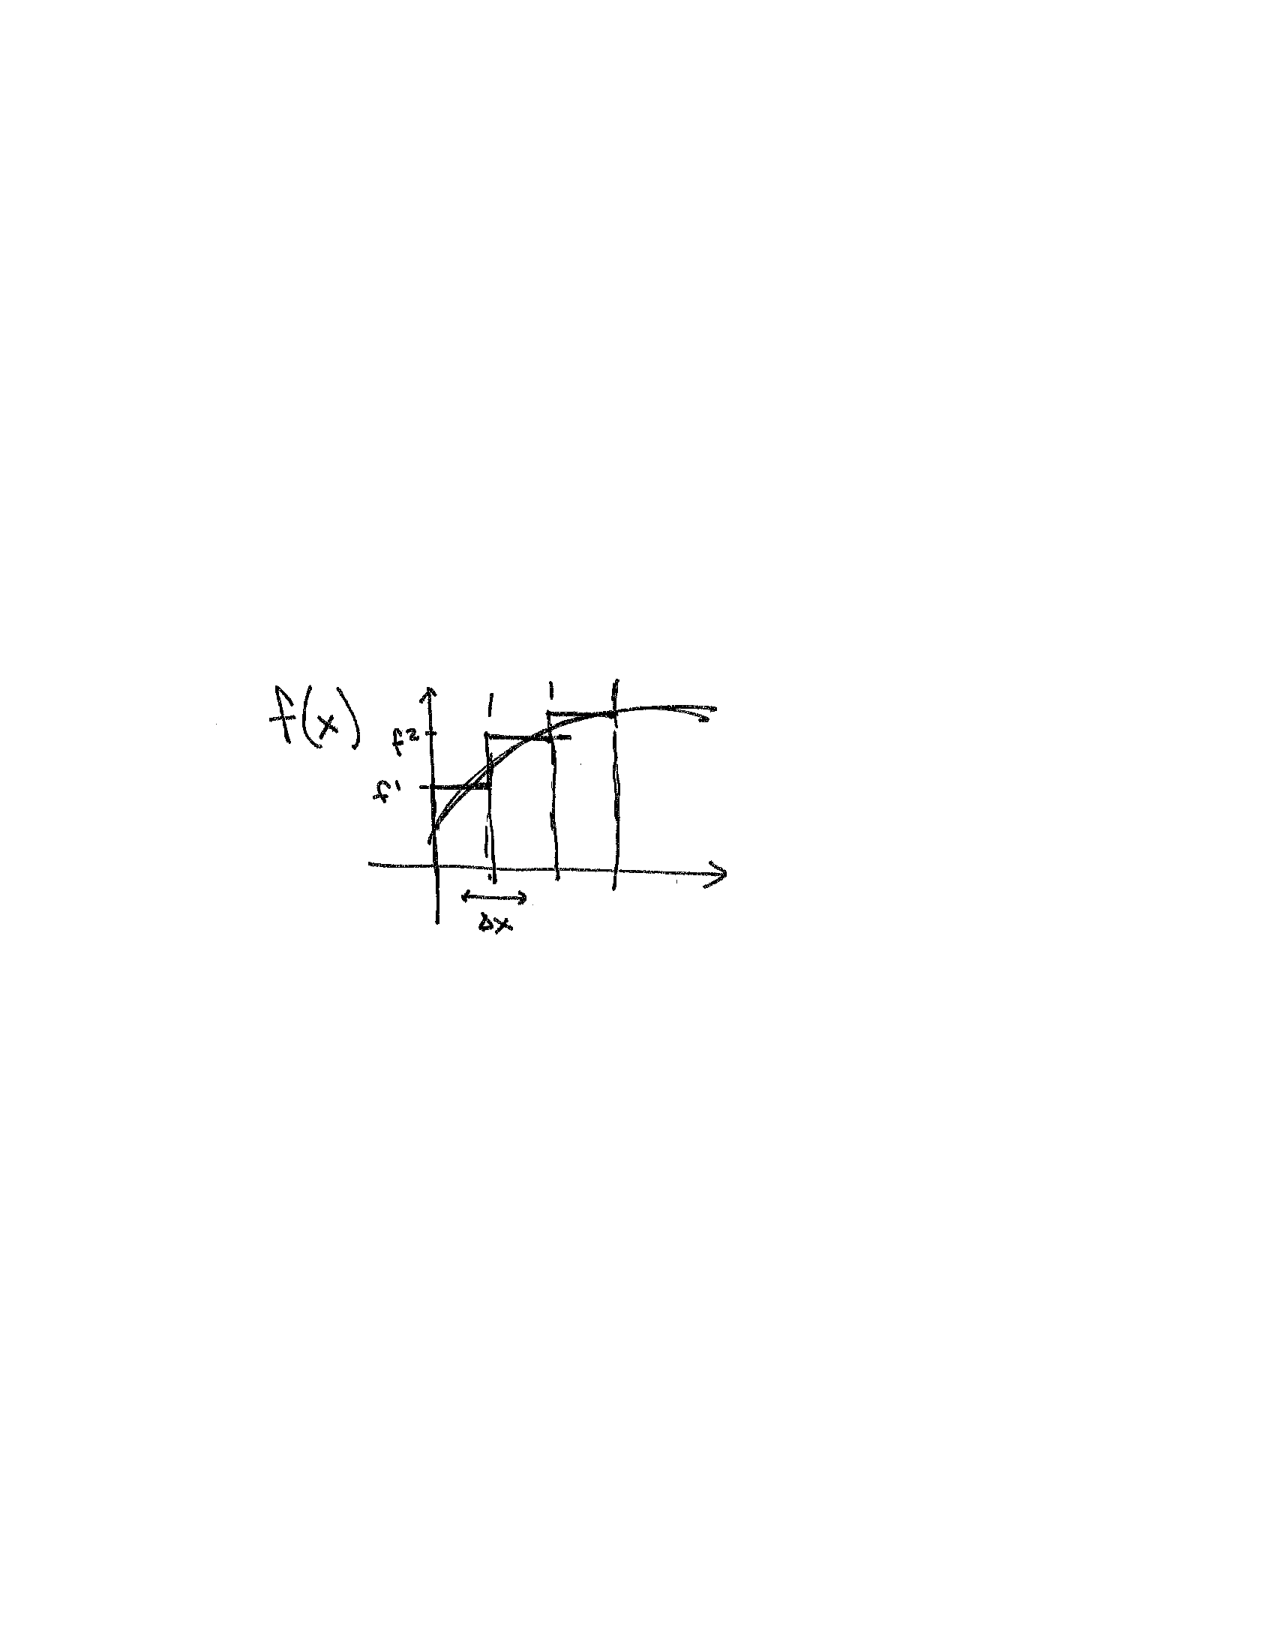
\includegraphics[width=.4\textwidth]{figures/lec02_histfun.pdf}
\end{center}

Thus a vector in this approximate (discretized) \emph{function} space is 
\begin{align}
  \vec{f} = 
  \begin{pmatrix}
    f^1 \\
    f^2 \\
    \vdots\\
    f^N
  \end{pmatrix} \ .
\end{align}

\subsection{Derivative Operators}

Our discretized function space allows us to define a [forward] derivative:
\begin{align}
  \vec{f'} =
  \frac{1}{\Delta x}
  \begin{pmatrix}
    f^2 - f^1 \\
    f^3 - f^2 \\
    \vdots
    \\
    f^{i+1}-f^i
    \\
    \vdots
  \end{pmatrix} \ .
\end{align}
This is familiar if you’ve ever had to manually program a derivative into a computer program. Note that the right-hand side looks like a linear transformation of $\vec{f}$. In other words, we expect to be able to write a matrix $D$ so that
\begin{align}
  \vec{f'} = D\vec{f} \ .
\end{align}
One problem is apparent: what happens at the `bottom’ of the vector? What is the last component of the derivative, $\vec{f'}^N$? Formally, this is
\begin{align}
  {(f')}^N = \frac{1}{\Delta x}(f^{N+1} - f^N) \,
\end{align}
but now we have no idea what $f^{N+1}$ is. That was never a component in our vector space. There is no $\vec{e}_{(N+1)}$ basis vector. 

This demonstrates and important lesson that we’ll need when we move more formally to function spaces: \emph{boundary conditions are part of the definition of the function space}. 

In the present case, let’s assume Dirichlet boundary conditions. A convenient way to impose this is to define what happens to all functions outside the domain of the function space:
\begin{align}
  f^{i > N} = f^{i < 1} = 0 \ .
\end{align}
This solves the problem of the derivative on the last component:
\begin{align}
  {(f')}^N = \frac{1}{\Delta x}(f^{N+1} - f^N) 
  = 
  \frac{- f^N}{\Delta x}  \ .
\end{align}

Alternatively, we could have also imposed periodic boundary conditions:
\begin{align}
  f^{i} &= f^{i+ kN}
  & k\in \mathbb{Z} \ .
\end{align}
This would then give
\begin{align}
  {(f')}^N = \frac{1}{\Delta x}(f^{N+1} - f^N) 
  = 
  \frac{1}{\Delta x}(f^{1} - f^N) 
  \ .
\end{align}
One could have also defined a backward derivative where $(f')^i \sim f^{i}-f^{i-1}$ \ . The second derivative may be defined symmetrically:
\begin{align}
  (f'')^i = \frac{(f^{i+1} - f^i) - (f^i - f^{i-1})}{\Delta x^2} \ .
\end{align}
You may pontificate about the reason why the first derivative does have a symmetric discretization while the second derivative does. 


\subsection{Derivatives in other function space bases}

There are other ways to write a discrete basis of functions. Here’s a natural one for functions that are up to second-order polynomials:
\begin{align}
  \vec{e}_{(0)} &= 1
  &
  \vec{e}_{(1)} &= x
  &
  \vec{e}_{(2)} &= x^2 \ .
\end{align}
Let’s sidestep questions about orthonormality for the moment. Clearly linear combinations of these basis functions can produce any quadratic function:
\begin{align}
  f(x) &= a x^2 + bx + c
  & \Rightarrow&&
  \vec{f} &=
  \begin{pmatrix}
     c \\ b \\ a
   \end{pmatrix} \ . 
\end{align}
The derivative operator has an easy representation in this space:
\begin{align}
  D = 
  \begin{pmatrix}
    0 & 1 & 0   \\
    0 & 0 & 2   \\
    0 & 0 & 0   
  \end{pmatrix} \ .
\end{align}
We can see that
\begin{align}
  D \vec{f}  &= 
  \begin{pmatrix}
     b \\
     2 a \\
     0
  \end{pmatrix} 
  &
  D^2 \vec{f}  &= 
  \begin{pmatrix}
     2a \\
     0 \\
     0
  \end{pmatrix} 
  &
  D^3 \vec{f}  &= 
  0 \ .
\end{align}
The last line is, of course, the realization that the third-derivative of a quadratic function vanishes. Feel free to attach mathy words to this like \emph{kernel}.

There are other bases that we may use for function space. A particularly nice one that we will use over and over is the Fourier basis, which we prosaically refer to as \emph{momentum space}. The basis vectors are things like sines, cosines, or oscillating exponentials. These do not vanish for any power of $D$.


\subsection{Locality}


\subsection{Row Vectors and all that}

In high school we didn’t distinguish between row vectors and column vectors. They both seemed to convey the same information. The row vectors were just `tipped over.’ Perhaps you noticed that they follow the rules of `matrix multiplication’ act on a vector:
\begin{align}
  \begin{pmatrix}
    w_1 & w_2 & \cdots
  \end{pmatrix}
  \begin{pmatrix}
    v^1 \\
    v^2 \\
    \vdots
  \end{pmatrix}
  &= 
  w_1 v^1 + w_2 v^2 + \cdots \ .
\end{align}
In fact, this is like $\vec{w}^T$ is a function that acts linearly on $\vec{v}$: 
\begin{align}
  \vec{w}^T(\vec v) &= w_1 v^1 + w_2 v^2 + \cdots \ .
\end{align}

Indeed, let is be a bit more formal about this. This layer of formalism is uncharacteristic of our approach in this course, but this underpins so much of the mathematical structure of our physical theories that it is worth getting right from the beginning. 

Let $V$ be a vector space. It contains vectors, $\vec{v}$. Sometimes these are called contravariant vectors or kets. They have basis vectors $\vec{e}_{(i)}$. 

Now introduce a related but \emph{completely distinct} vector space called $V^*$. This is the space of \textbf{dual vectors} to $V$. A \textbf{dual vector} is what you may know as a \textbf{row vector}, a \textbf{ket}, a \textbf{covariant vector}, or a [differential] \textbf{one-form}. These are all words for the \emph{same idea}. An element of $V^*$, say $(\vec{w}^T)$ is a linear function that takes vectors and spits out numbers:
\begin{align}
  \vec{w}^T \in V^* \Rightarrow \vec{w}^T: V \to \mathbb{R} \ .
 \end{align}
Don’t think about $\vec{w}^T$ as some kind of operation on a vector $\vec{w}\in V$; at least not yet. For now the `$^T$' is just part of the name of $\vec{w}^T$. The two spaces $V$ and $V^*$ are totally different. We haven’t said anything about how to turn elements of $V$ into elements of $V^*$ or vice versa.
%
It should be clear that there is a sense of `duality’ here: the vectors $V$ are also linear functions that take a dual vector and spit out a number. 

Let us call the basis of dual vectors $\tilde{\vec{e}}^{(i)}$. This notation is cumbersome, so we’ll change to something different soon. The upper index is deliberate. The defining property of $\tilde{\vec{e}}^{(i)}$ is:
\begin{align}
  \tilde{\vec{e}}^{(i)}\left(\vec{e}_{(j)}\right) \equiv \delta^i_j \ .
\end{align}
One may check that this gives
\begin{align}
  \left(w_i\tilde{\vec{e}}^{(i)}\right)\left(v^j\vec{e}_{(j)}\right)
  = w_i v^j \delta^i_j = w_i v^i = w_1 v^1 + w_2 v^2 + \cdots \ .
\end{align}



\subsection{Orthonormal Bases}

At this point we should take a deep breath and state explicitly that we’ve been assuming an orthonormal basis. In this course we will continue to use an orthonormal basis. You may object to this and say that you used to believe in orthonormal bases until you had to write down the gradient (or worse, the Laplacian) in spherical coordinates. 

There are many things to be said about this, none of them are particularly edifying without a full discussion. With no apologies, I’ll make the following [perhaps perplexing] remarks:
\begin{enumerate}
\item There is no such thing as a `position vector.' Positions refer to some base space, whereas vectors (like differential operators) act on the tangent space at a point of that base space. 
\item A given tangent space is `nice’ and has a nice orthonormal basis. 
\item That basis may not be the same for neighboring tangent spaces (perhaps due to coordinates, perhaps due to intrinsic curvature). 
\end{enumerate}
In this course these nuances will not come up. In the rest of your life you’ll still have to deal with curvilinear coordinates. But suffice it to say that our study of function space will be nice an orthonormal. Of course, we haven’t yet given a definition of `normality.’

\subsection{Bra-Ket Notation}

There is neither any physics nor mathematics contained in a choice of notation. However, a convenient notation does simplify our lives. Let us introduce bra-ket notation. In this notation, we denote vectors by kets:
\begin{align}
  |v\rangle = v^i|i\rangle \ ,
\end{align}
where $|i\rangle = \vec{e}_{(i)}$ is the basis of vectors that span the vector space $V$. There is nothing new or different about this object,  $\vec{v} = |v \rangle$.

We denote dual vectors (row-vectors, one-forms) as bras:
\begin{align}
  \langle w | &= w_i \langle i| \ ,
\end{align}
where $\langle i | = \tilde{\vec{e}}^{(i)}$. The orthonormality of this basis is encoded in 
\begin{align}
  \langle i | j \rangle = \delta^i_j \ .
\end{align}

In bra-ket notation a linear transformation $A$ has a basis
\begin{align}
  A = A^i_{\phantom{i}j} |i\rangle \langle j| \ .
\end{align}
The notation $|i\rangle \langle j|$ is shorthand for $|i\rangle \otimes \langle j|$. If the $\otimes$ doesn’t mean anything to you, that’s fine. It doesn’t mean much to me either. Matrix multiplication proceeds as before:
\begin{align}
  A\vec{v} = A|v\rangle = 
  A^i_{\phantom{i}j} |i\rangle \langle j| v^k |k \rangle
  = 
  A^i_{\phantom{i}j}  v^k  |i\rangle \langle j|k \rangle
  = 
  A^i_{\phantom{i}j}  v^k  |i\rangle \delta^j_k
  = 
  A^i_{\phantom{i}j}  v^j  |i\rangle \ .
\end{align}
Observe that the power of the notation is clear: the object with the index $v^i$ is just a number. It commutes with everything. All of the vector-ness is carried in the basis objects: the bras, kets, and ket-bras. Those do not commute. But they have a well defined way in which kets act on bras (or vice versa).\footnote{This is where the $\oplus$ notation is handy. It keeps track of which kets/bras might hit which other bras/kets. This falls under the name of multi-linear algebra.}


\subsection{Eigenvectors are nice}

Give a sufficiently \emph{nice} linear transformation, $A$, there is a particularly convenient basis: the eigenvectors of $A$. These are kets $|\lambda\rangle$ such that
\begin{align}
  A |\lambda\rangle = \lambda |\lambda\rangle \ .
\end{align}
In other words, $A$ acts on the eigenvector by rescaling. The rescaling coefficient is the eigenvalues. For \emph{nice} transformations, there is a complete set of such vectors to span the vector space.

If you write a general vector $|v\rangle$ in terms of this eigenbasis,
\begin{align}
  |v\rangle = v^i |\lambda_{(i)} \rangle \ ,
\end{align}
Then the action of $A$ on this vector is easy:
\begin{align}
  A |v\rangle = \sum_i \lambda_{(i)} v^i |\lambda_{(i)} \rangle \ .
\end{align}
In fact, assuming that all of the eigenvalues are non-zero, even the matrix inverse is easy:
\begin{align}
  A^{-1}|v\rangle = \sum_i \lambda_{(i)}^{-1} v^i |\lambda_{(i)} \rangle \ .
\end{align}


\subsection{The Green’s Function Problem}

Going back to the big picture: recall that we want to solve differential equations of the form $\mathcal O f(x) = s(x)$. If we had a sense of the \emph{eigenfunctions} of $\mathcal O$, then we could expand $s(x)$ in a basis of those eigenfunctions and then apply $\mathcal O^{-1}$ to both sides. 

The analog is this:

\begin{center}
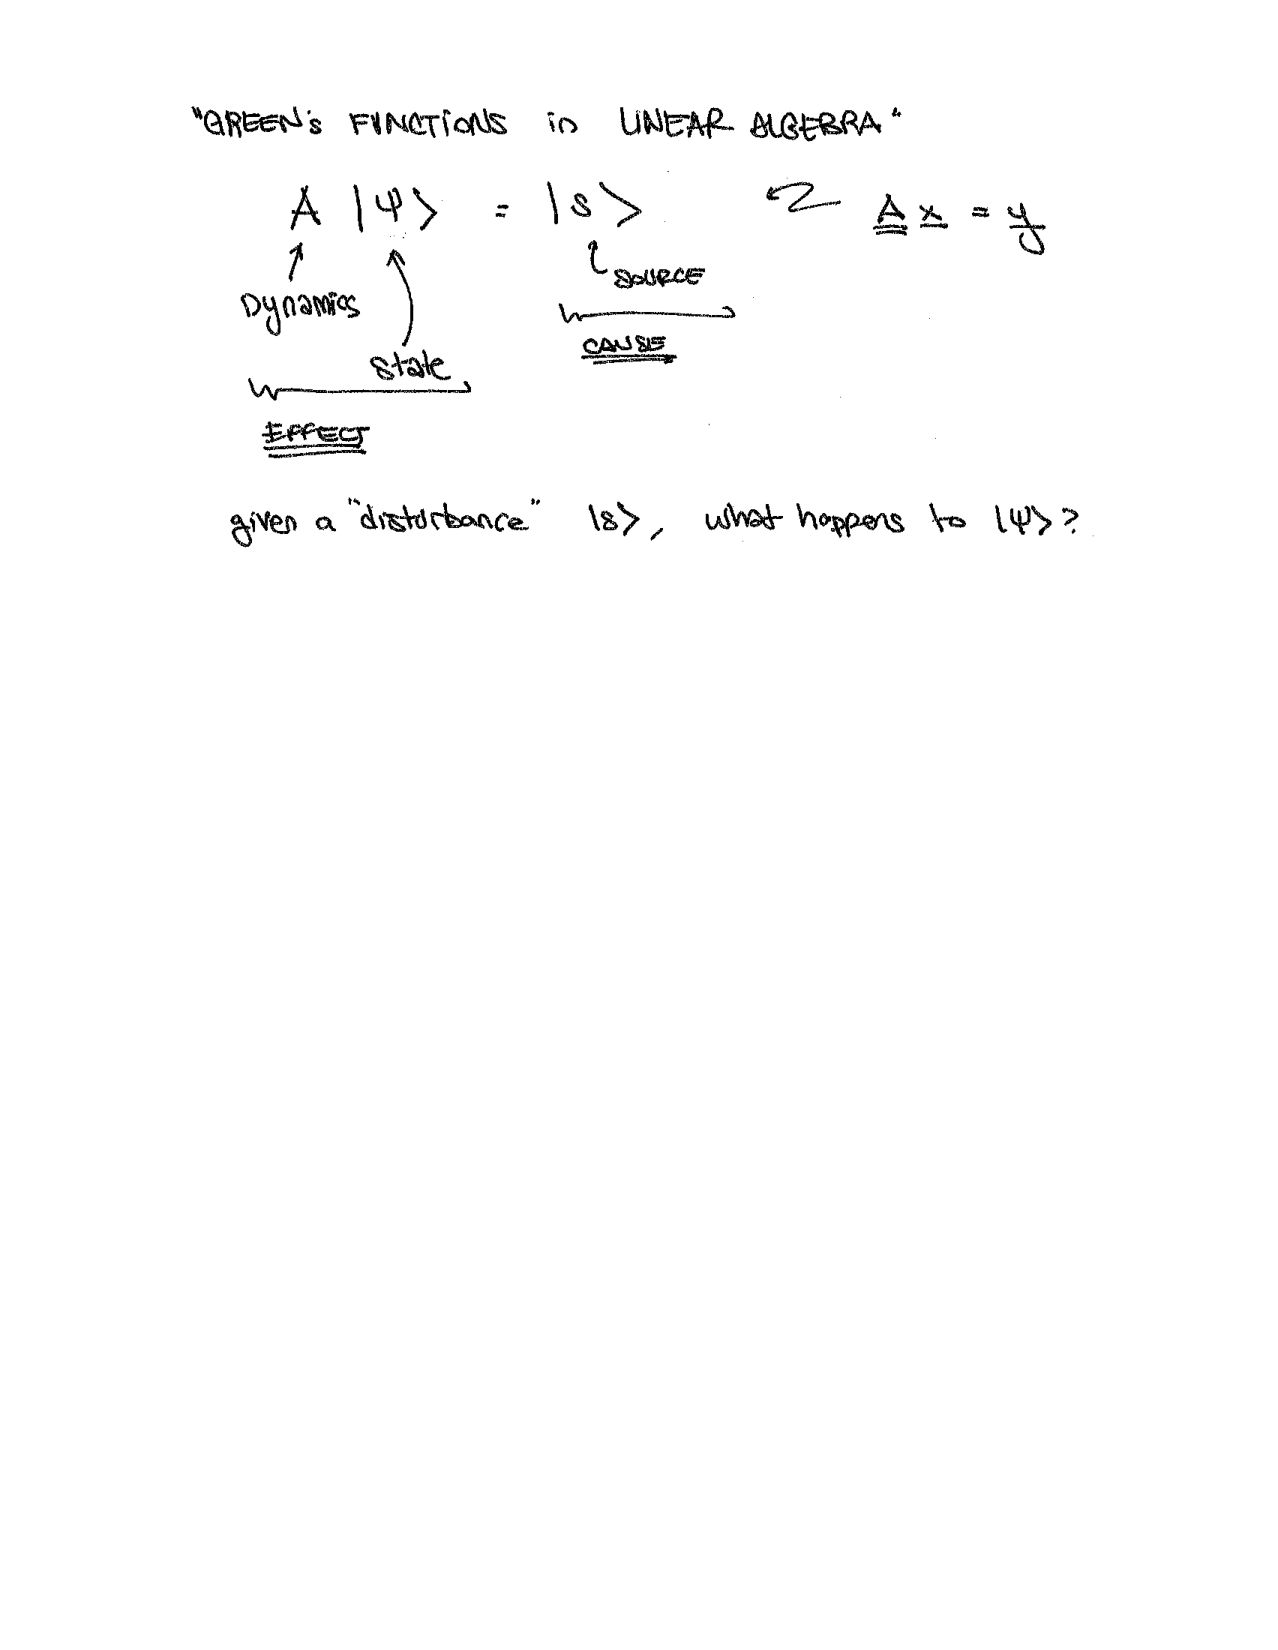
\includegraphics[width=.7\textwidth]{figures/lec02_green01.pdf}
\end{center}

The operator $A$ encodes the \emph{physics} of the system, the underlying dynamics.
%
This is presumably local: it is a near-diagonal matrix coming from one or two powers of derivatives.  The ket $|s\rangle$ is the source. This is the thing that \emph{causes} the dynamics. The ket $|\psi\rangle$ is some state that we would like to determine. 

\subsection{Metrics}

Thus far we have introduced vector spaces. The dual vector space is a set of linear functions that act on elements of a vector space; these are bras/row-vectors/one-forms. Let us now introduce a new piece of machinery: a \textbf{metric}. This is also known as an \textbf{inner product} or a \textbf{dot product}. A space with a metric is called a metric space. We only state this fact to emphasize that we are \emph{adding this structure by hand}. Vector spaces don‘t come with metrics---someone makes up a metric and slaps it onto the vector space.

The \textbf{metric} is a function that takes two vectors and spits out a number. It is linear in each argument. In other words, a metric $g$ is:
\begin{align}
  g:\; V\times V\to \mathbb{R} \ .
\end{align}
Occasionally one may want a metric defined such that the output is a complex number. We thus have:
\begin{align}
  g(\alpha \vec{v} + \beta\vec{w}, \delta \vec{x} + \gamma \vec{y})
  &= 
  \alpha \delta g(\vec{v},\vec{x}) + \alpha \gamma g(\vec{v},\vec{y}) + \beta\delta g(\vec{w},\vec{x}) + \beta\gamma g(\vec{w},\vec{y}) \ .
\end{align}
One more special assumption about the metric is that it is \textbf{symmetric}:
\begin{align}
  g(\vec{v},\vec{w}) = g(\vec{w}, \vec{v}) \ .
\end{align}
In indices one may write
\begin{align}
  g &= g_{ij} \langle i | \otimes \langle j |
\end{align}
so that
\begin{align}
  g(\vec{v}, \vec{w}) = g_{ij} v^{i}w^j \ .
 \end{align}
 Here we see the usefulness of the $\otimes$ notation. It tells us that the bras and kets resolve as follows:
 \begin{align}
   g_{ij}\langle i | \otimes \langle j | \left(v^k|k\rangle\right)\left(w^\ell|\ell\rangle\right) 
   = 
   g_ij v^k w^\ell 
   \langle i | k\rangle \langle j |\ell\rangle
   = 
   g_ij v^k w^\ell  \delta^i_k \delta^j_\ell 
   = 
   g_{ij} v^{i}w^j \ .
 \end{align}
 For ordinary Euclidean space in flat coordinates, the metric is simply the unit matrix: $g_{ij} = \text{diag}(1,\cdots, 1)$. In Minkowksi space there’s a relative minus sign between space and time. In curvilinear coordinates things get ugly. 
 
Here’s the neat thing about metrics. We can take a metric and pre-load it with a vector. Given a metric $g$ and a vector $\vec{v}$, we may define a function
\begin{align}
  g(\vec v,\qquad ) \ .
\end{align}
This is simply means that the function $f(\vec{w}) = g(\vec v,\vec w)$. Observe that $f(\vec{w})$ is a linear function that takes elements of $V$ and returns a number. In other words, this is a \emph{dual vector} (row-vector, one-form). Observe what having a machine like the metric has done for us: it has allowed us to convert vectors into dual vectors:
\begin{align}
  g(\vec v,\qquad )  = g_{ij} v^i \langle j| \ .
\end{align}

Similarly, one may define an inverse metric $g^{-1}$ such that $g^{-1}g = \mathbbm{1}$. In a slight abuse of notation, the inverse metric is written with two upper indices: $g^{ij}$. Note that we do not write the `$^{-1}$.' The inverse metric will \emph{raise} the index on a lower-index object, while the metric \emph{lowers} the index of an upper-index object.\footnote{Of course: what’s really happening is that the metric has a basis $\langle i|\otimes \langle j|$ while the inverse metric has a basis $|i\rangle \otimes |j\rangle$.}


\subsection{Hermitian Conjugate}

Now that we can go between column and row vectors, thanks to the metric and its inverse, it is worth thinking a bit about what we meant by the `transpose’ operator. The transpose precisely turned a column vector $\vec{v}$ into an associated column vector $\vec{v}^T$. The generalization of this idea is the Hermitian conjugate, $^\dag$. 










\section*{Acknowledgements}


%This work is supported in part by 
%the \textsc{nsf} grant \textsc{phy}-1316792. 
%
\textsc{p.t.}\ thanks 
\emph{your name here}
for useful comments and discussions. 
%
%\textsc{p.t.} thanks the Aspen Center for Physics (NSF grant \#1066293) for its hospitality during a period where part of this work was completed.

%% Appendices
% \appendix


%% Bibliography
%\bibliographystyle{utphys} 	% arXiv hyperlinks
%\bibliographystyle{utcaps} 	% arXiv hyperlinks
% \bibliography{bib title without .bib}


\end{document}